    
\section{TI nspire CX CAS}
	Matrix erstellen: "[\textbf{A}]", menu 7 1\\
	Spalte erweitern: "$\hookleftarrow$",  Zeile erweitern: "$\Uparrow$ shift" + "$\hookleftarrow$" \\
	\begin{tabular}{lll}
		\textbf{Zweck} & \textbf{Befehl} & \textbf{Text}\\
		Skalarprodukt & menu 7 C 3 & dotP($\vec{v}$, $\vec{v}$) \\
		Kreuzprodukt  & menu 7 C 2 & crossP($\vec{v}$, $\vec{v}$) \\
		Gauss, RREF & menu 7 5 & rref(\textbf{A}) \\
		Determinante & menu 7 3 & det(\textbf{A}) \\
		Matrix transponieren &  menu 7 2 & [\textbf{A}]$^t$\\
		Matrix invertieren & "$\wedge$" + "-1" & $[\text{\textbf{A}}]^{-1}$ \\
		Spur & menu 7 B 1 & trace(\textbf{A})\\
		LR-Zerlegung & menu 7 B 2 & LU \\
		QR-Zerlegung & menu 7 B 3 & QR \\
		Eigenwerte & menu 7 B 4 & eigVl(\textbf{A})\\
		Eigenvektoren & menu 7 B 5 & eigVc(\textbf{A}) \\
		Char. Polynom & menu 7 B 6 & charPoly(\textbf{A}, x) \\
	\end{tabular}
 
\section{Anwendungsbeispiele aus der Vorlesung}
		 %hier sind bewusst nur die Folien aus den Vorlesungen eingefügt, damit auf der ausgedrucken Form der Zusammenfassung individuelle Notizen gemacht werden können
		 
	\subsection{Matrixoptik}
		 
		 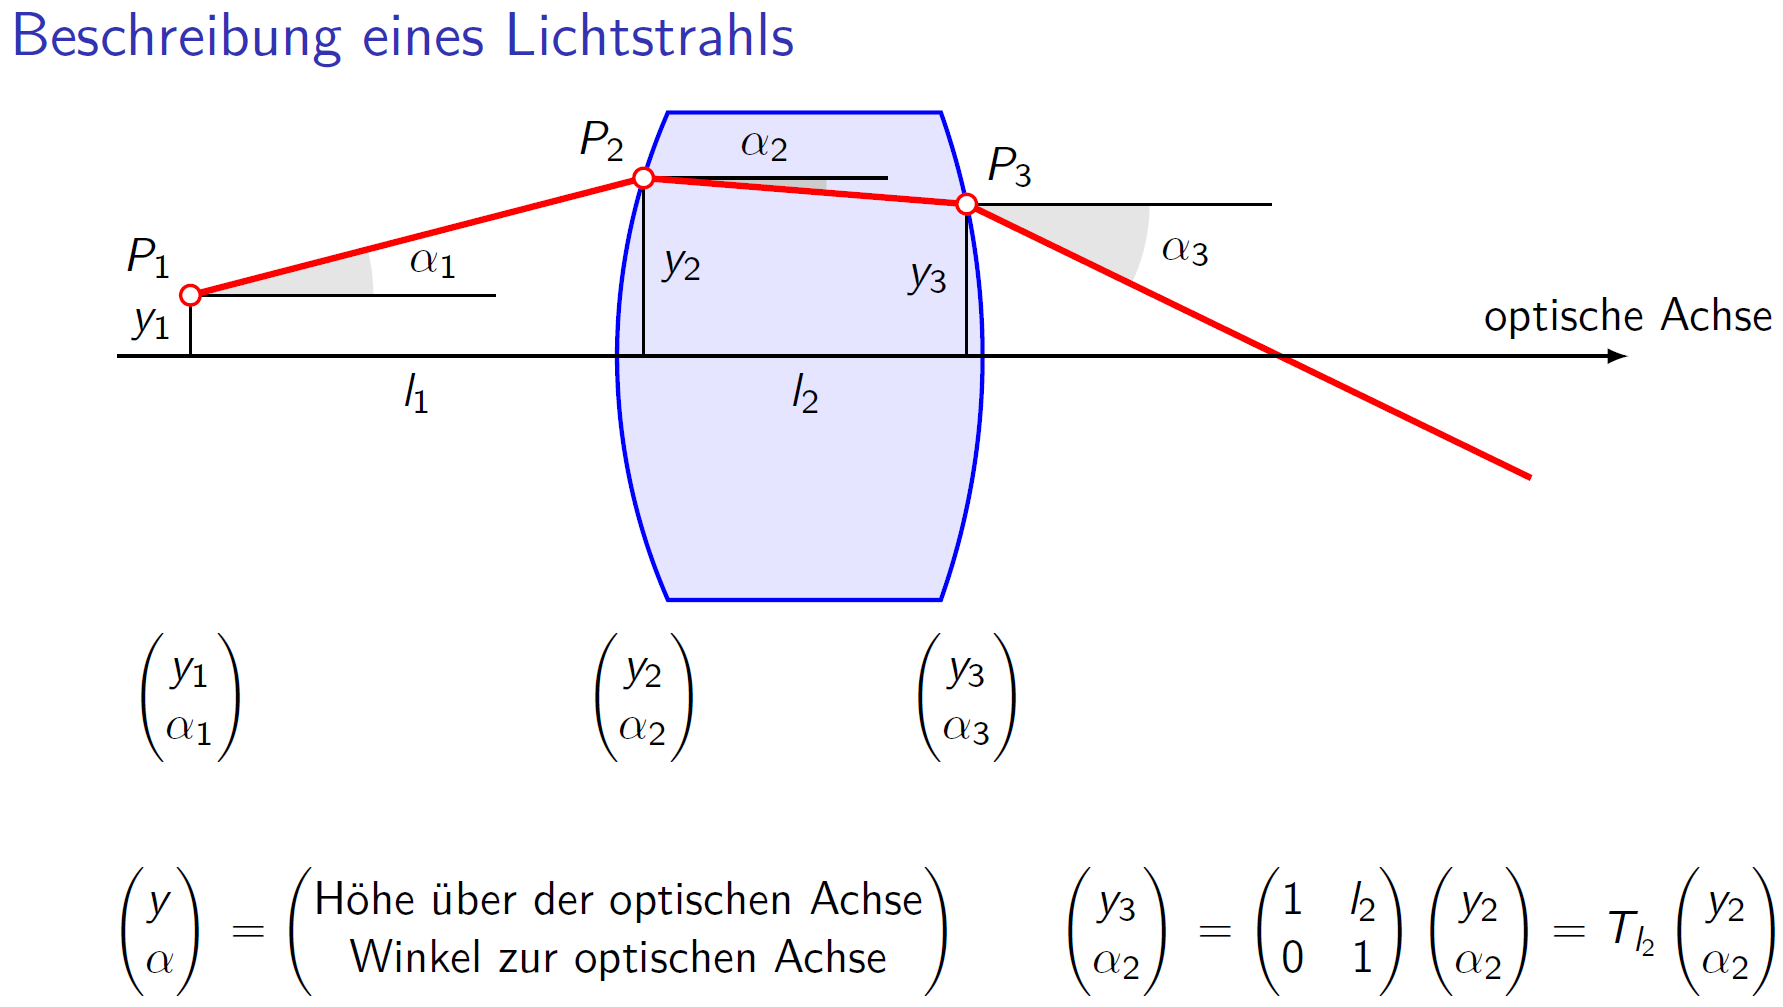
\includegraphics[width=0.85\linewidth]{Bilder/matrixoptik1} \\
		 
		 \vspace{0.5cm}
		 
		 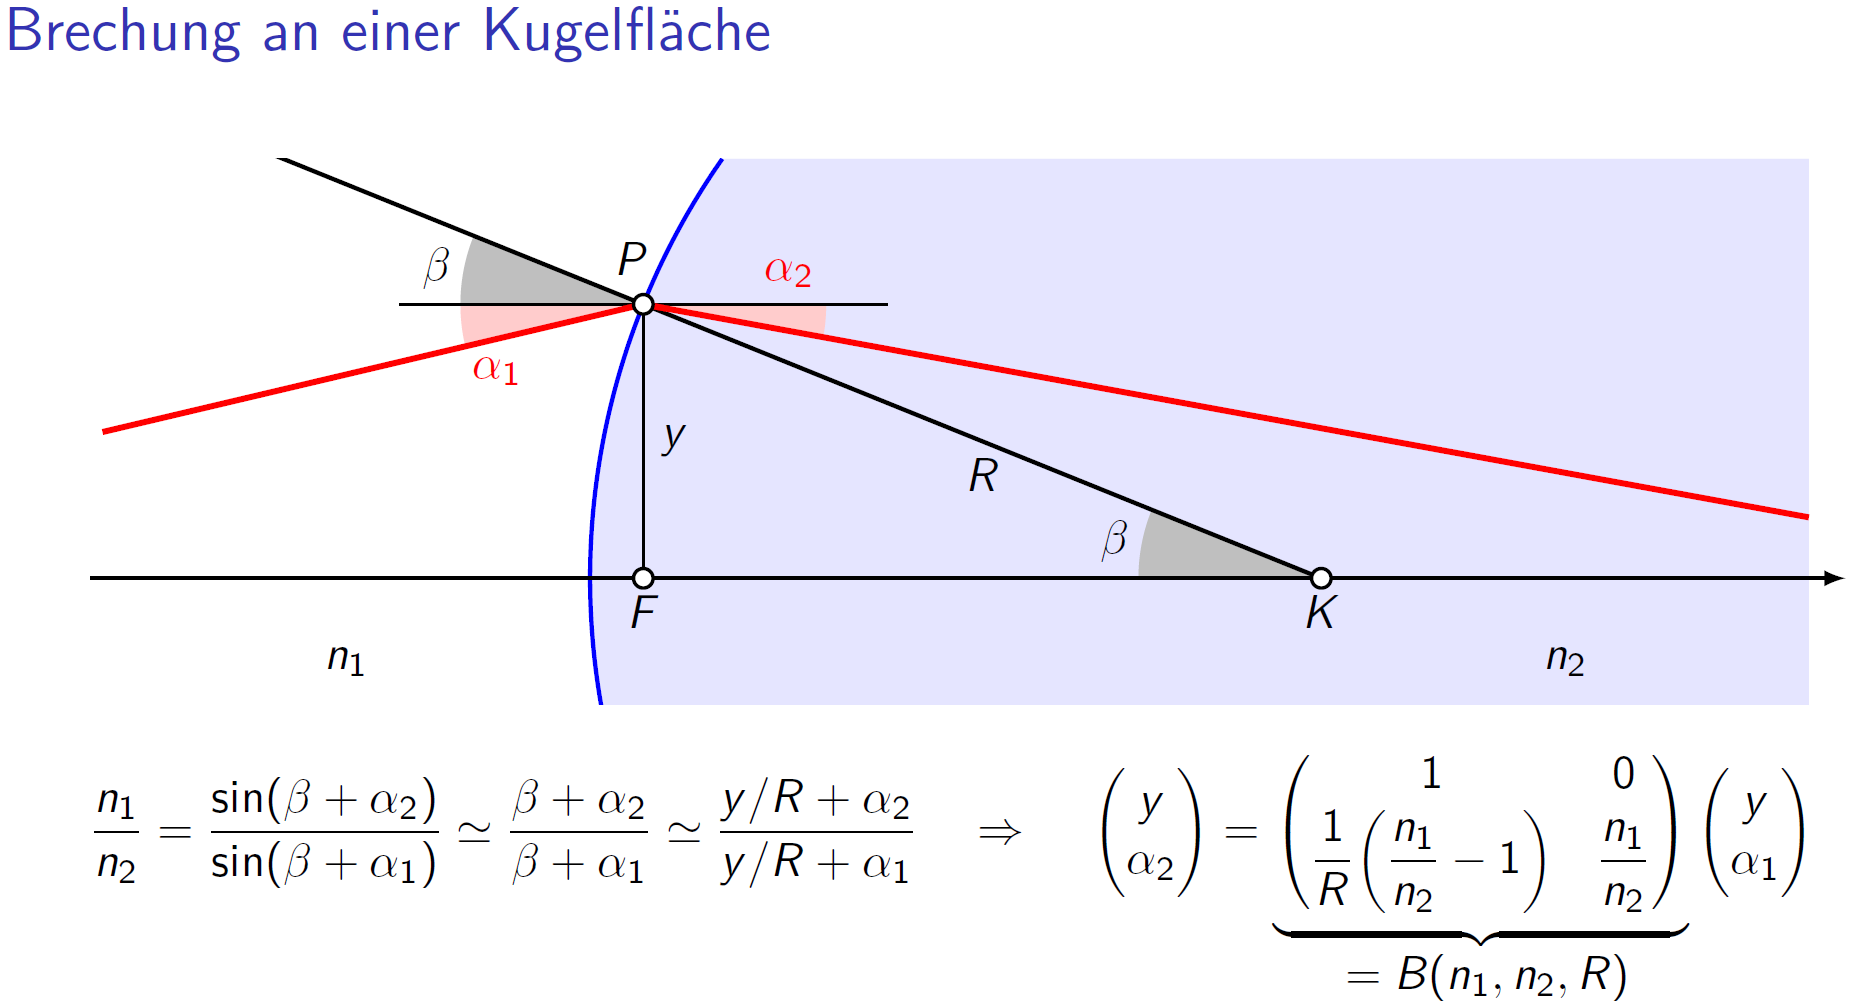
\includegraphics[width=0.85\linewidth]{Bilder/matrixoptik2} \\
		 
		 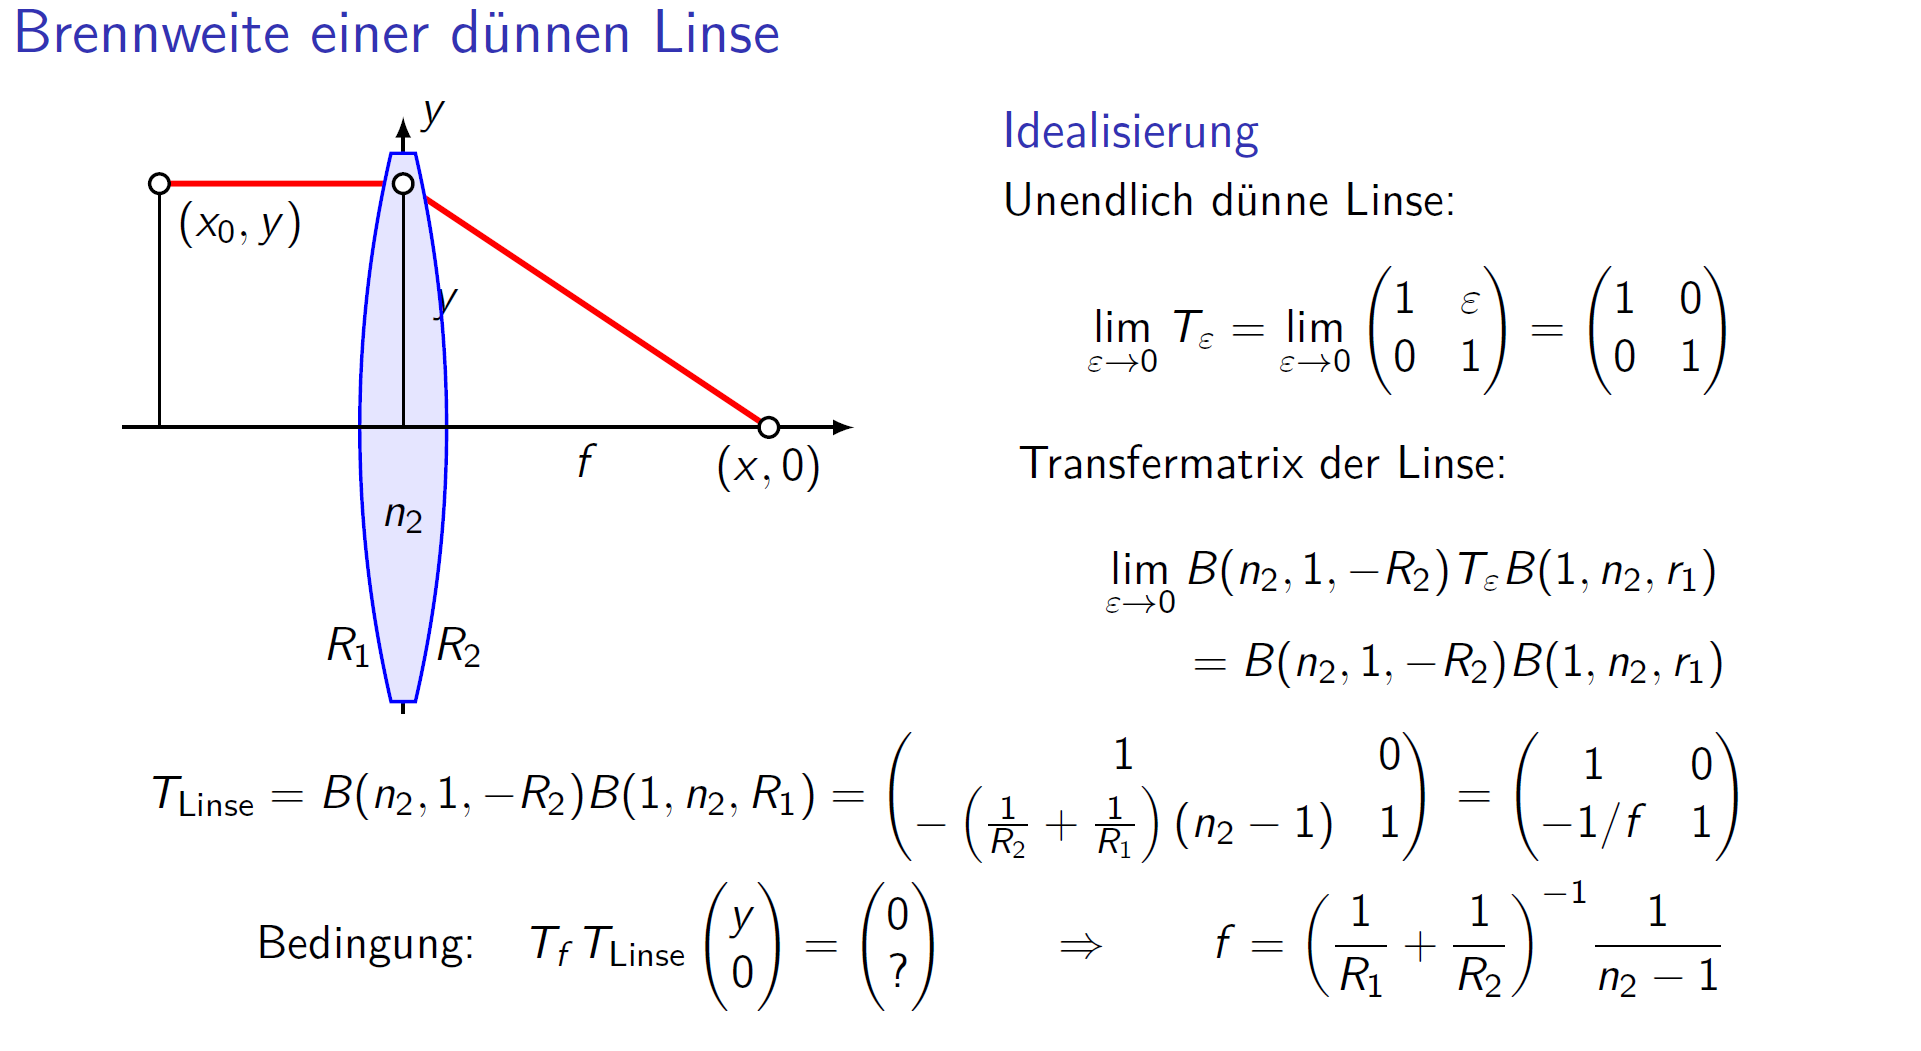
\includegraphics[width=0.8\linewidth]{Bilder/matrixoptik3} \\
		 
		 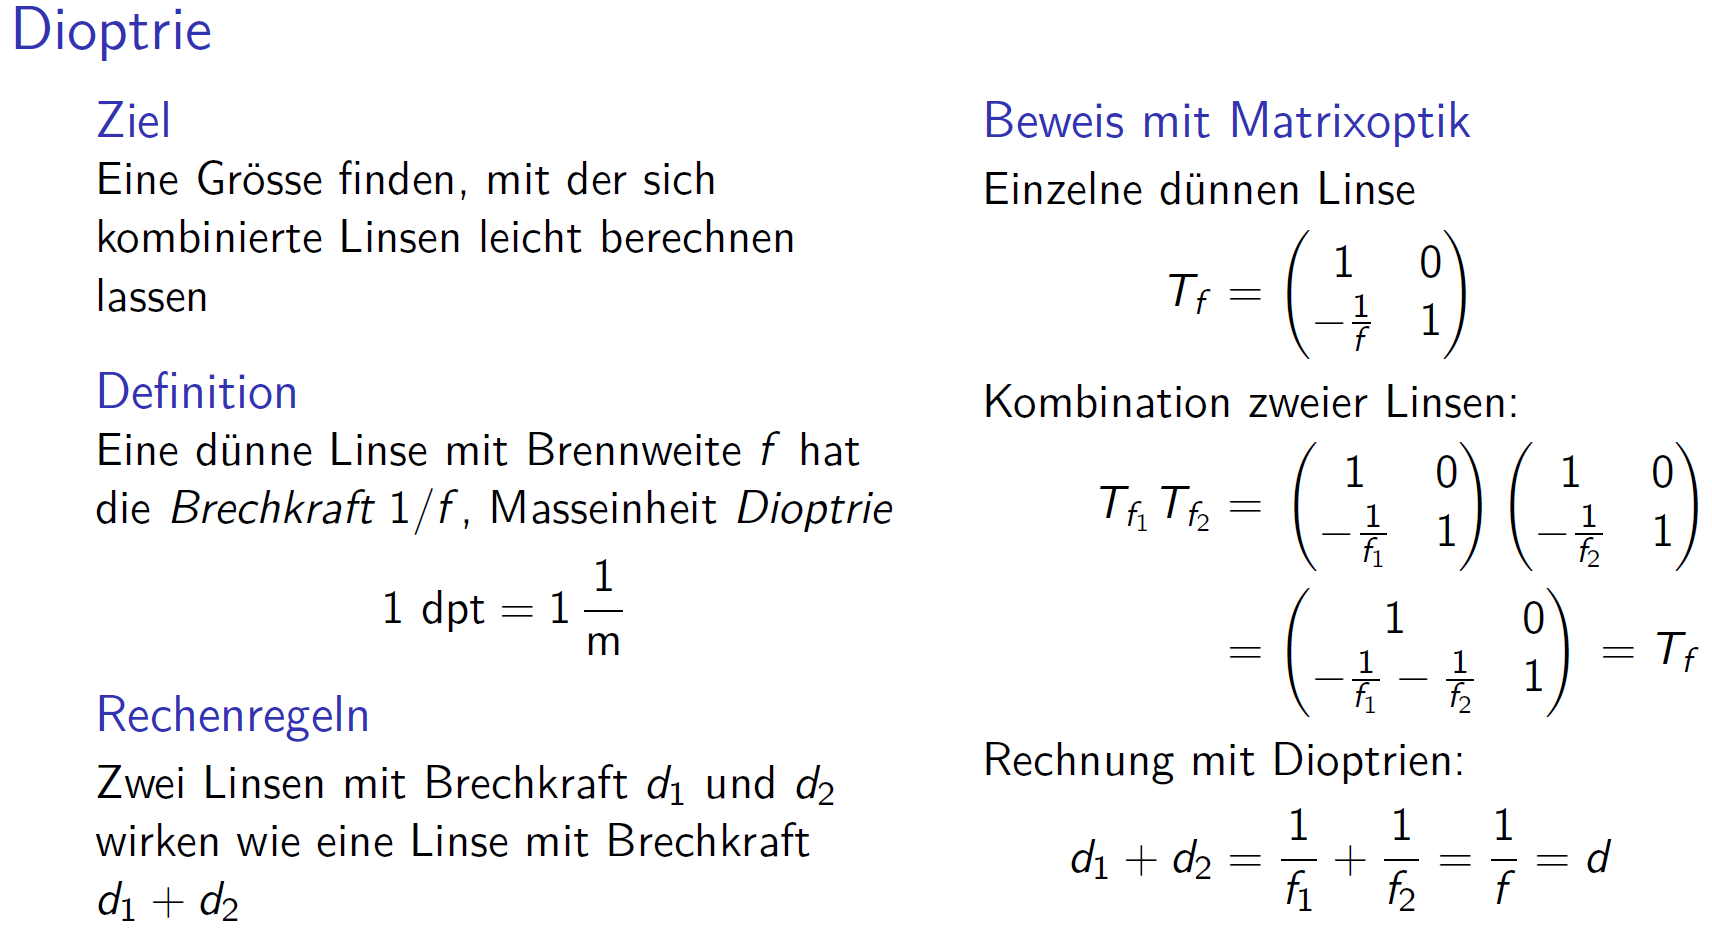
\includegraphics[width=0.8\linewidth]{Bilder/matrixoptik4} \\
		 
		 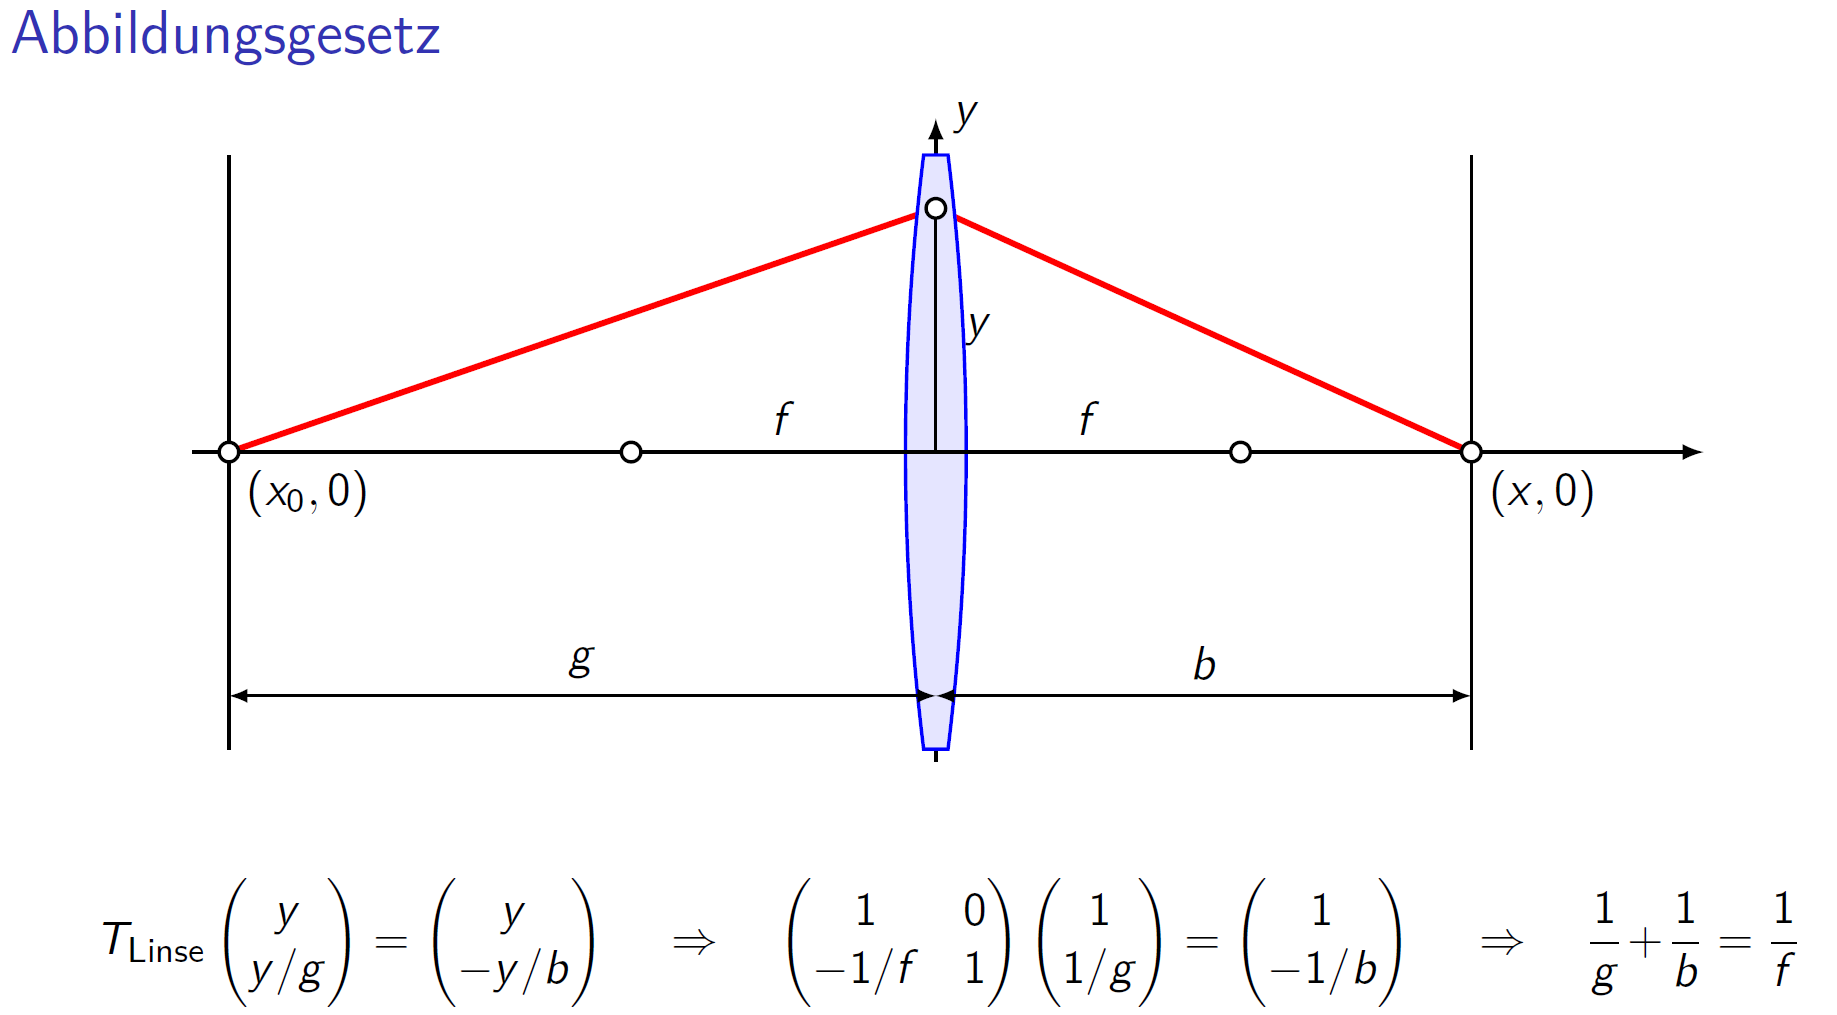
\includegraphics[width=0.8\linewidth]{Bilder/matrixoptik5}\\
		 
		 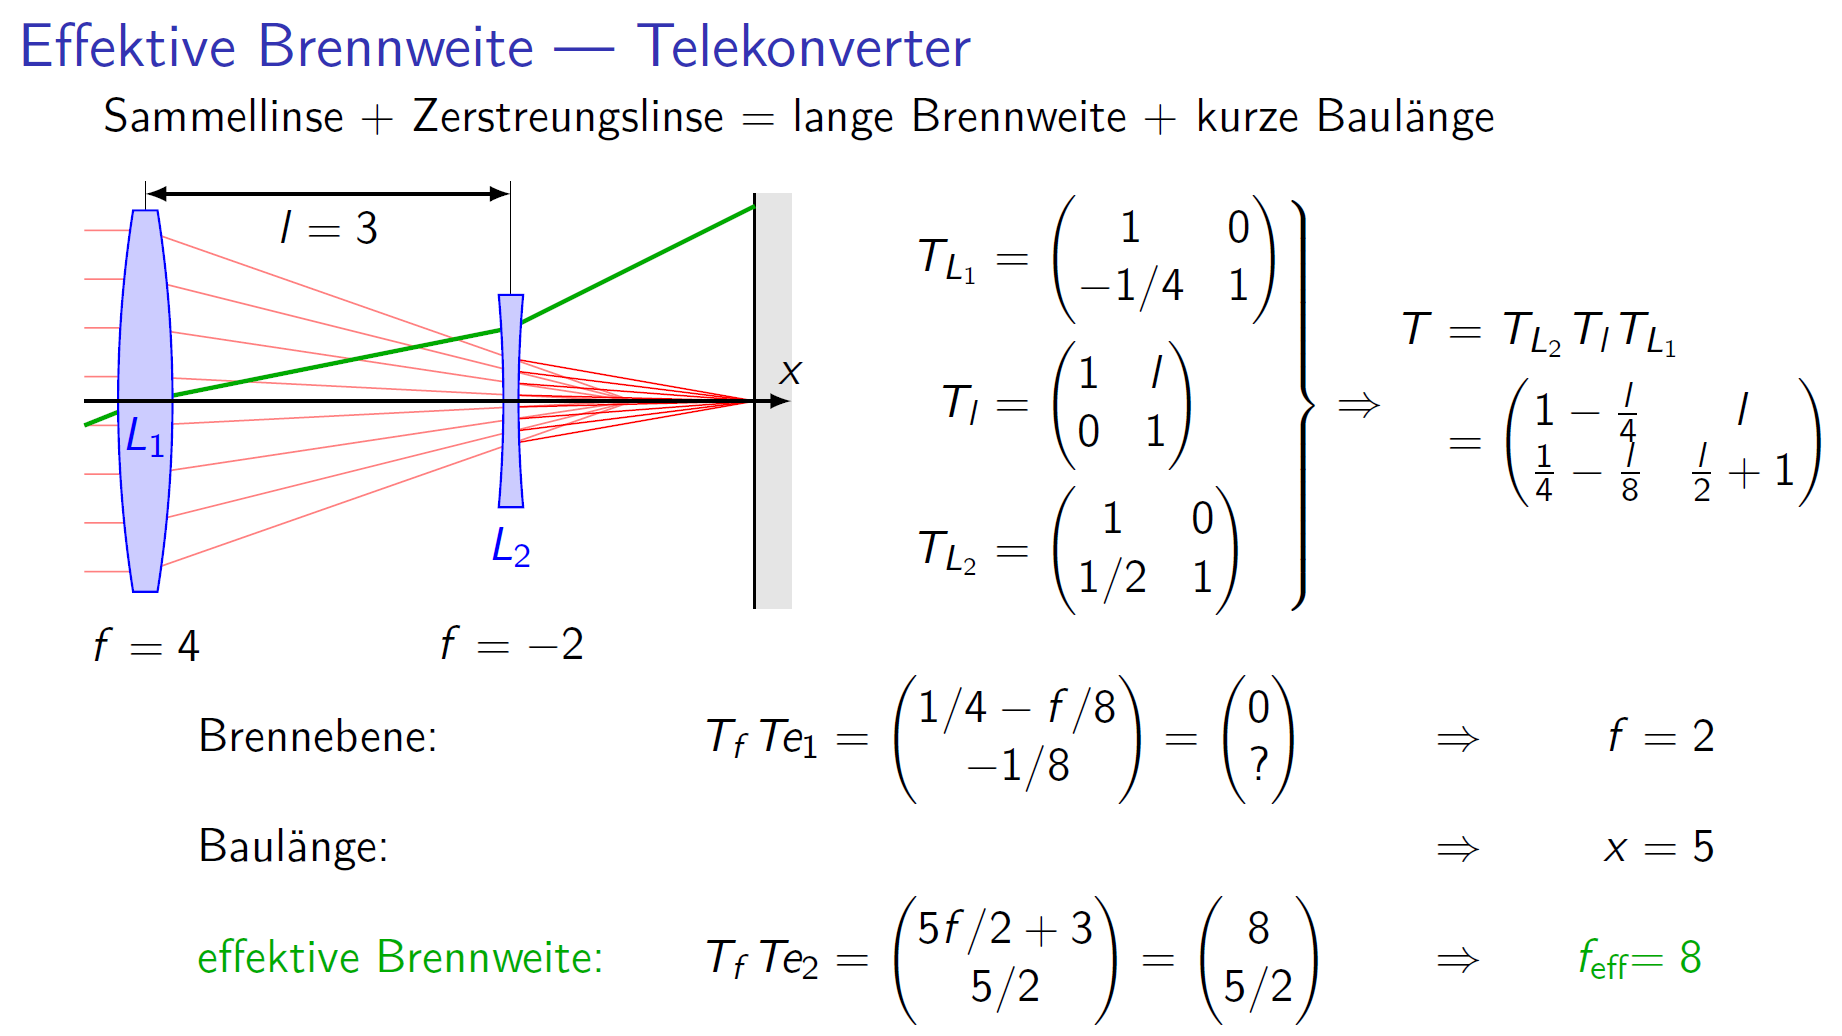
\includegraphics[width=0.8\linewidth]{Bilder/matrixoptik6} \\

	\subsection{Kettenbrüche}
		 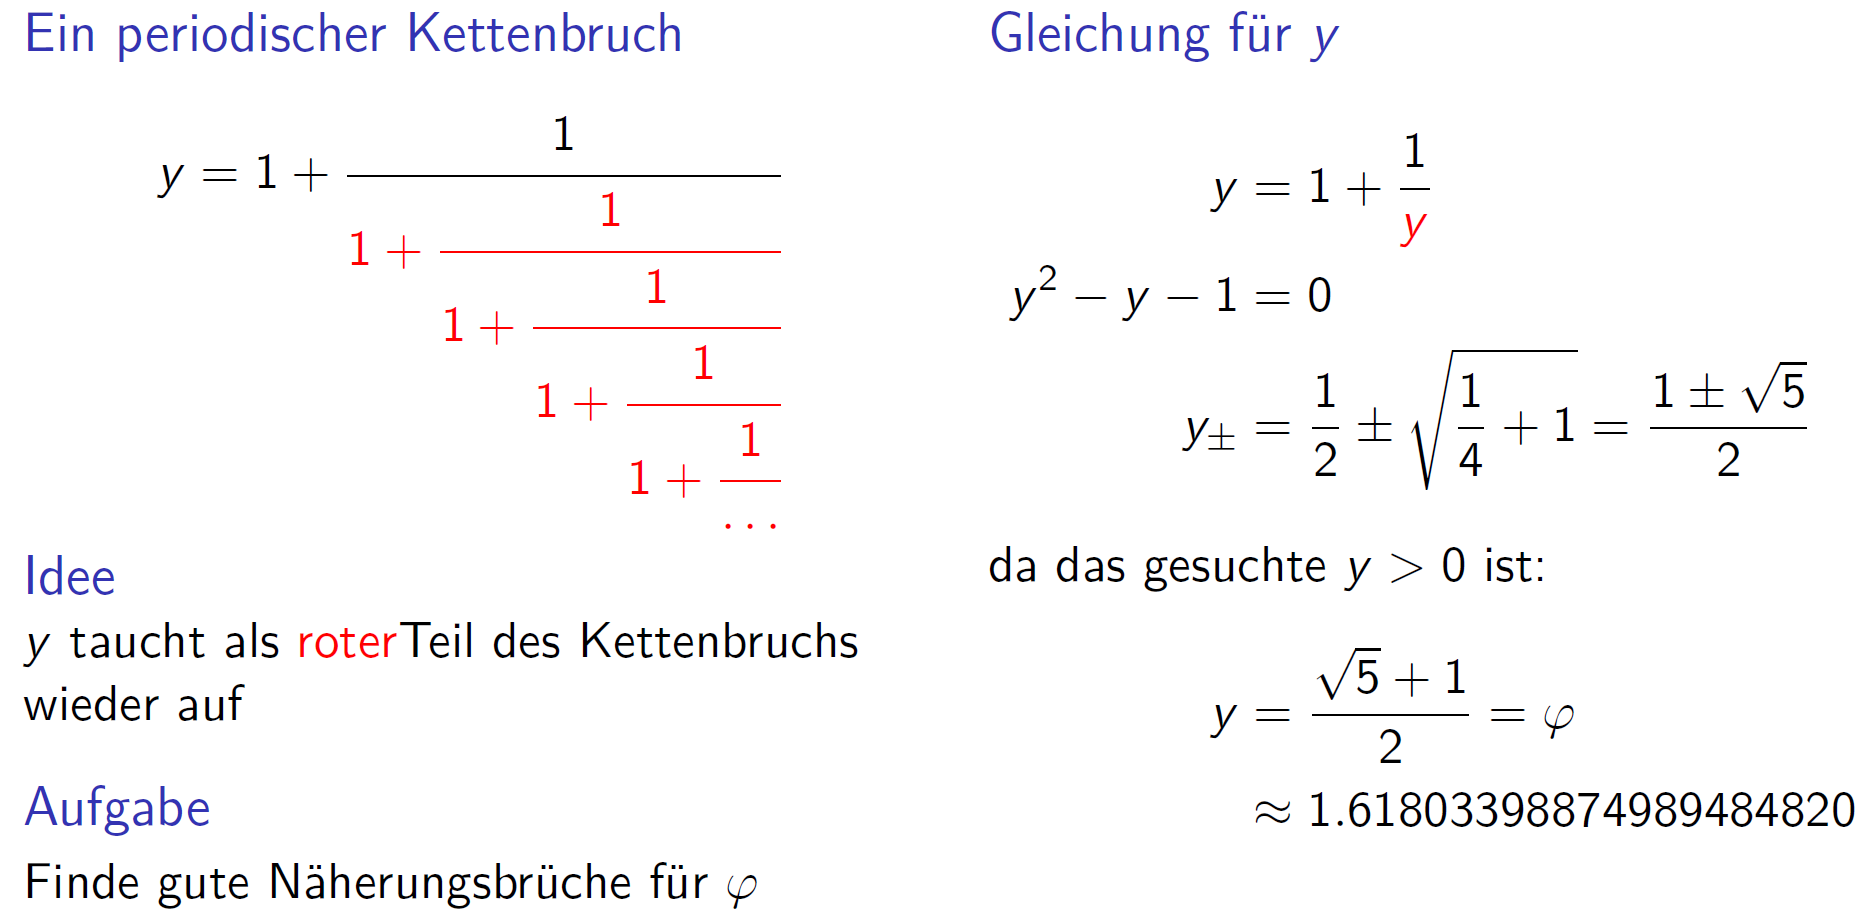
\includegraphics[width=0.8\linewidth]{Bilder/kettenbruch1} \\
		 
		 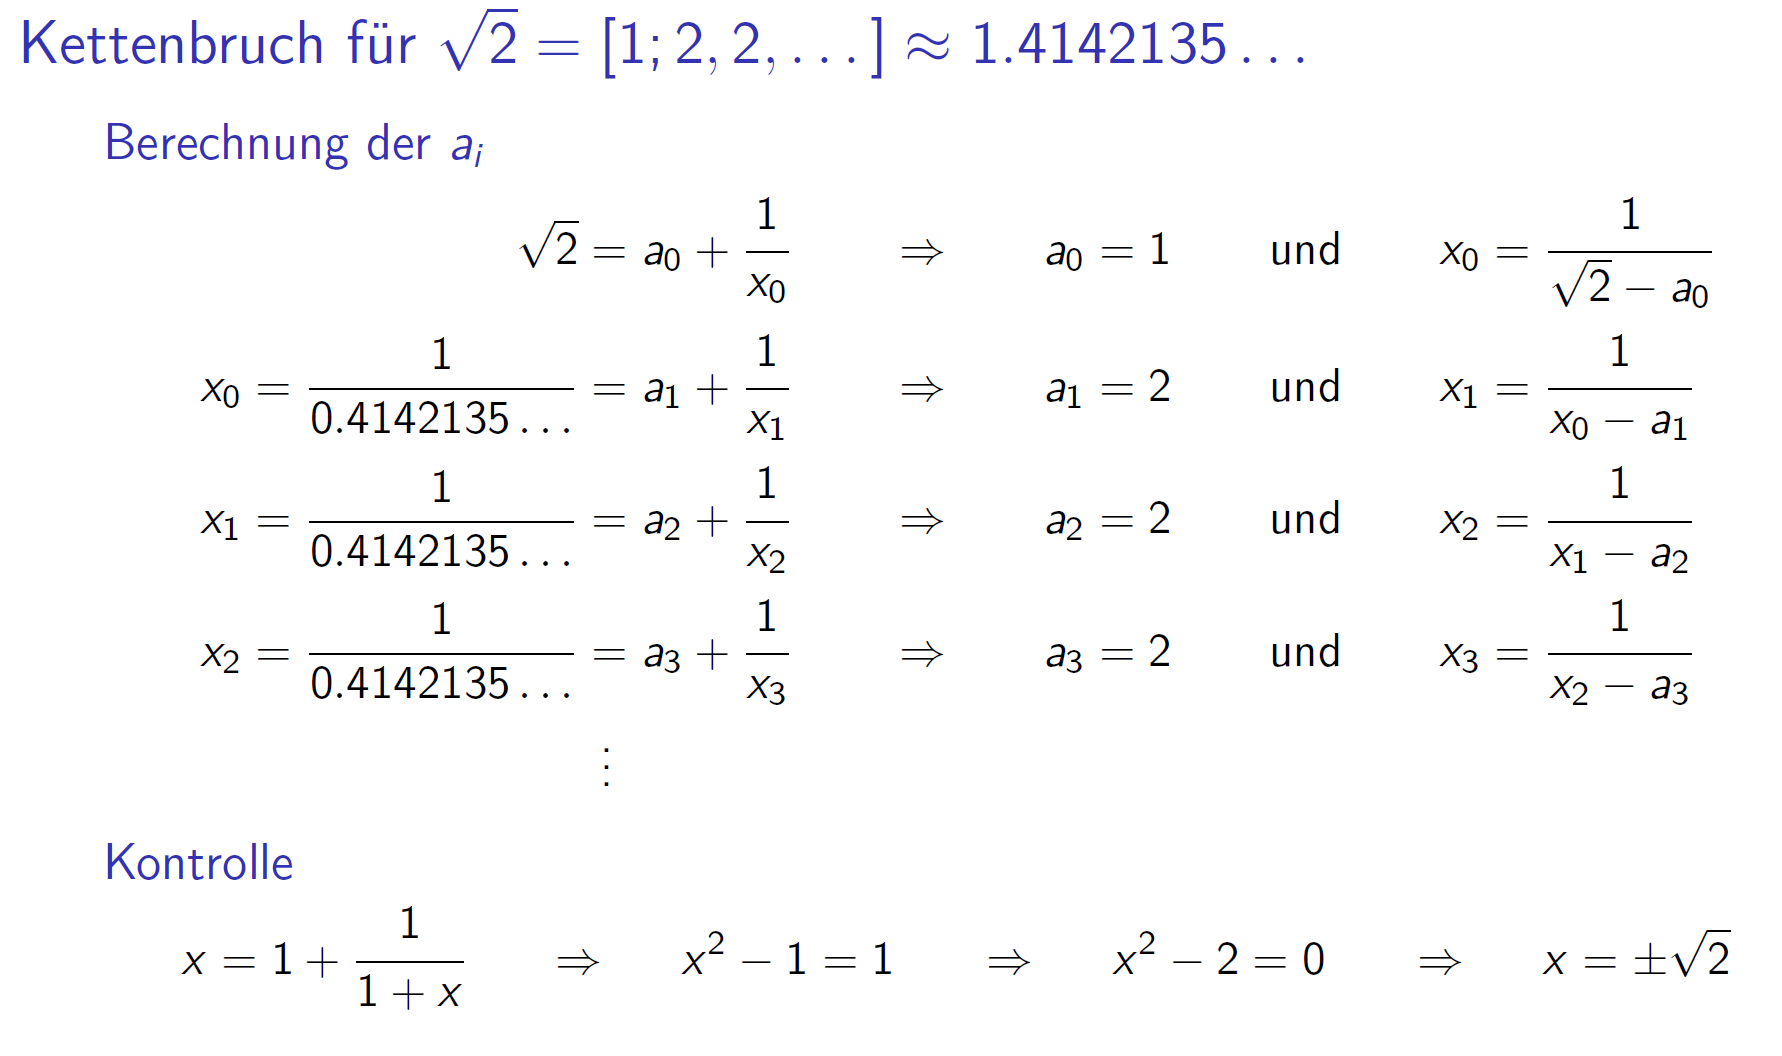
\includegraphics[width=0.8\linewidth]{Bilder/kettenbruch2} \\
		 
		 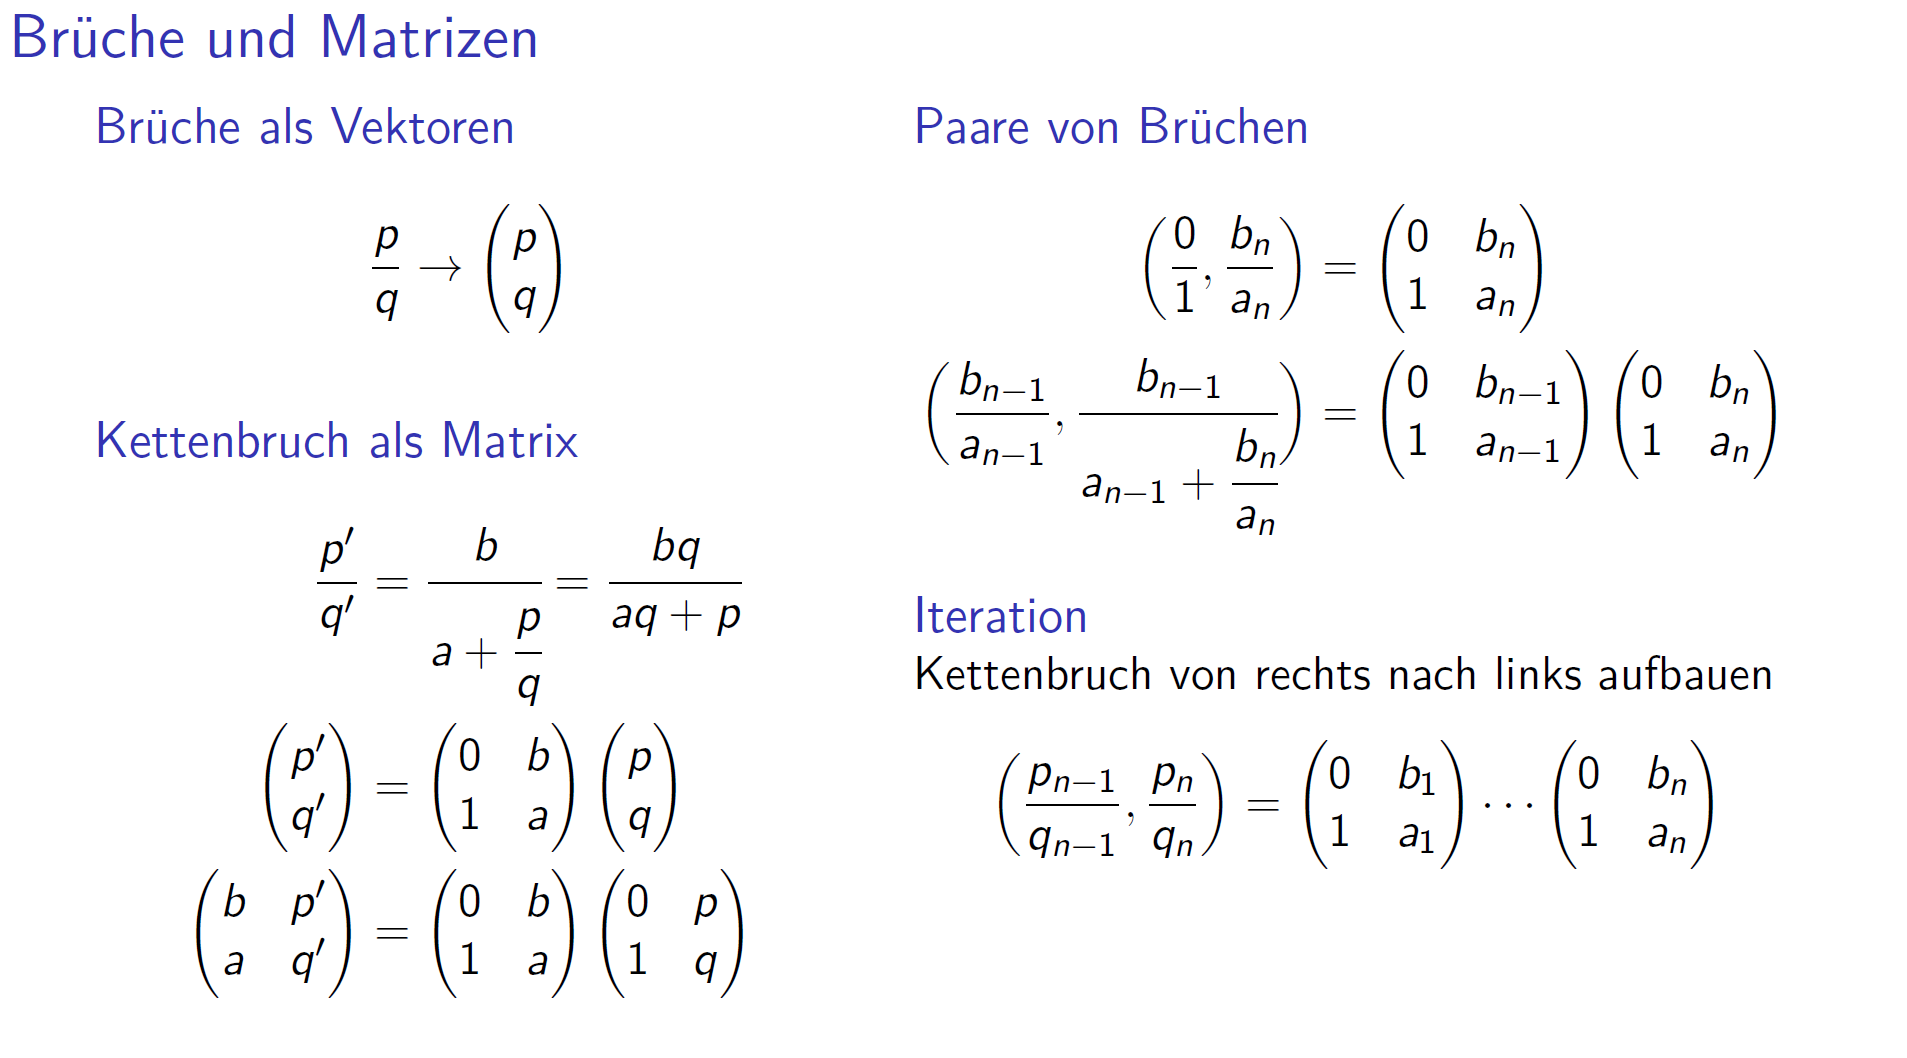
\includegraphics[width=0.8\linewidth]{Bilder/kettenbruch3} \\
		 
		 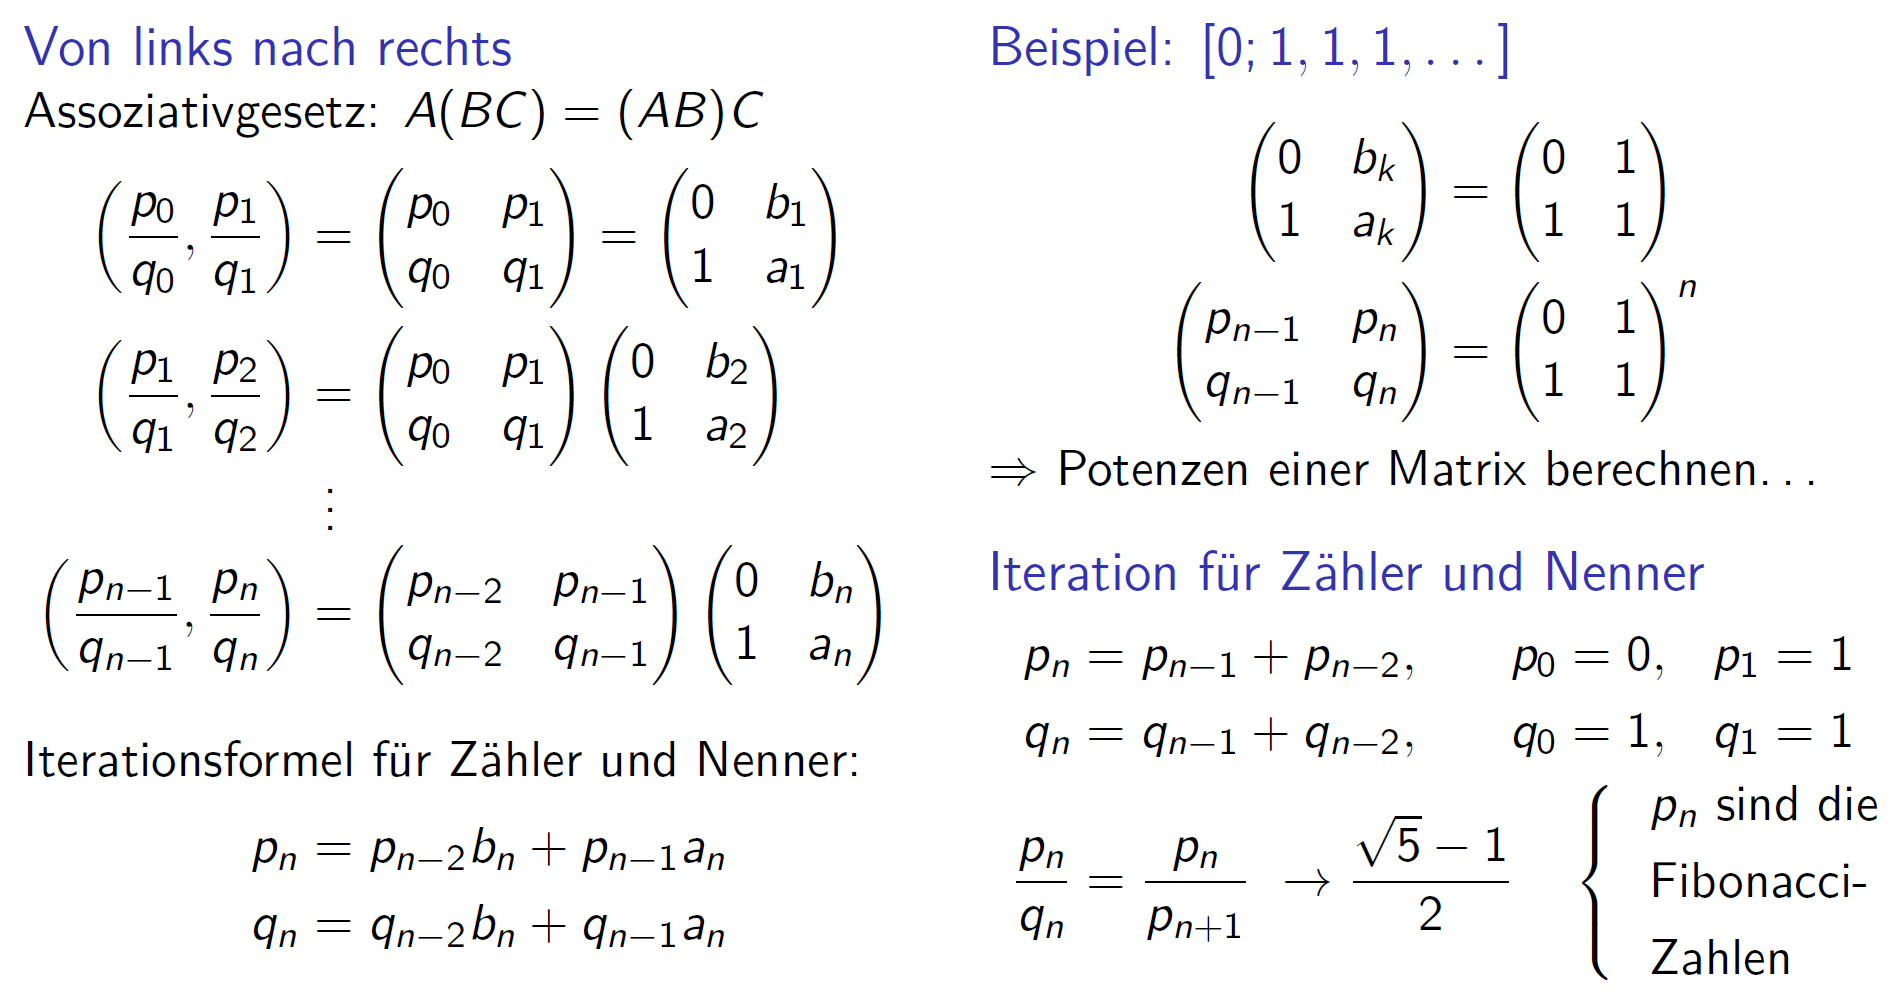
\includegraphics[width=0.8\linewidth]{Bilder/kettenbruch4} \\
		 
		 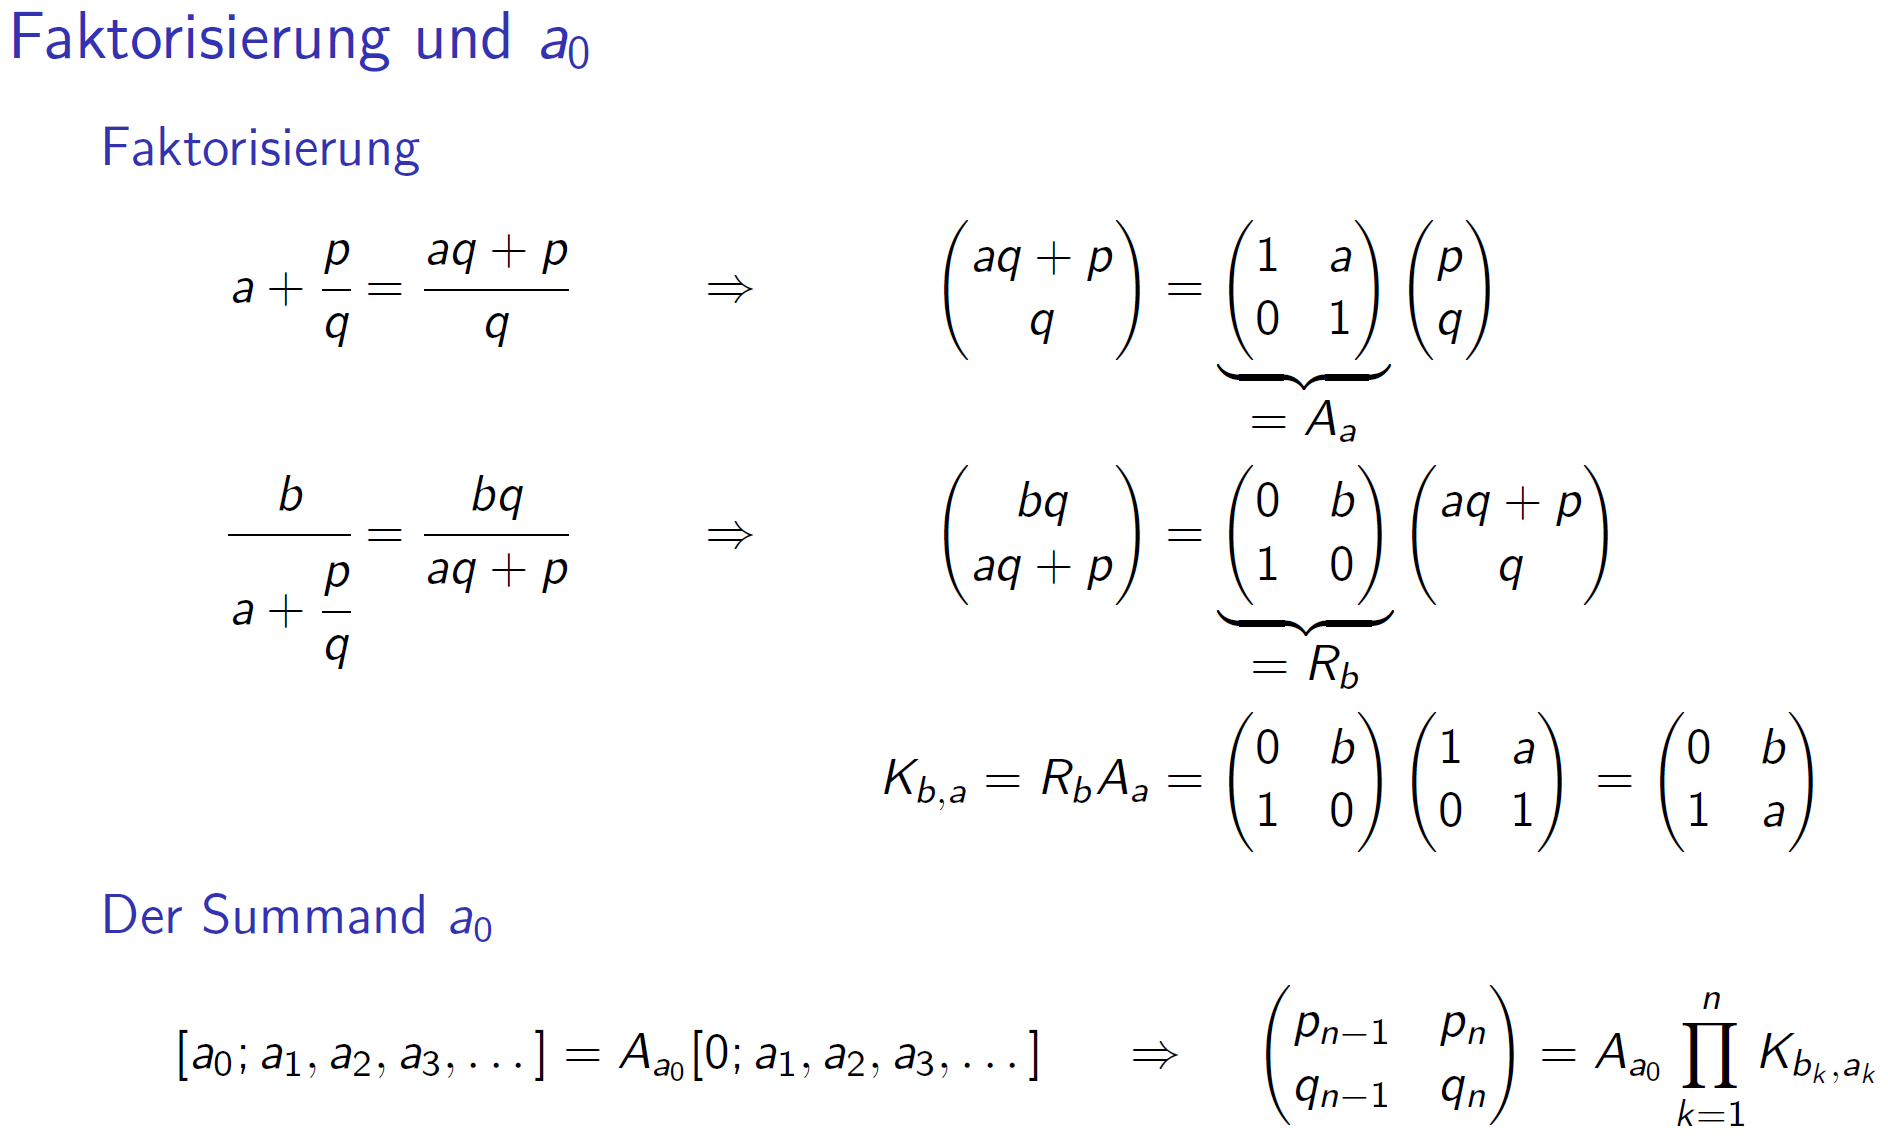
\includegraphics[width=0.8\linewidth]{Bilder/kettenbruch5} \\

	\subsection{Rekursionsformeln}
		 \textbf{Anwendung Eigenwerte / Eigenvektoren / Eigenbasis} \\
		 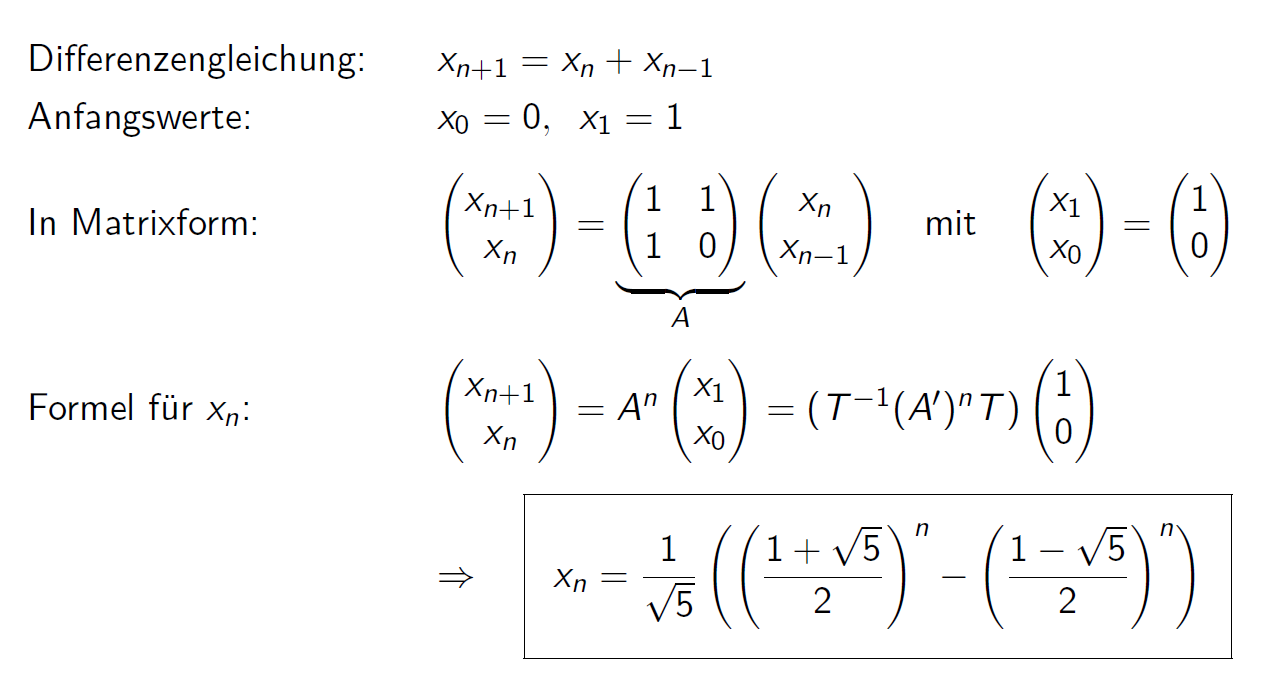
\includegraphics[width=0.8\linewidth]{Bilder/rekursion1} \\ 

	\subsection{Kamerageometrie}		 
		 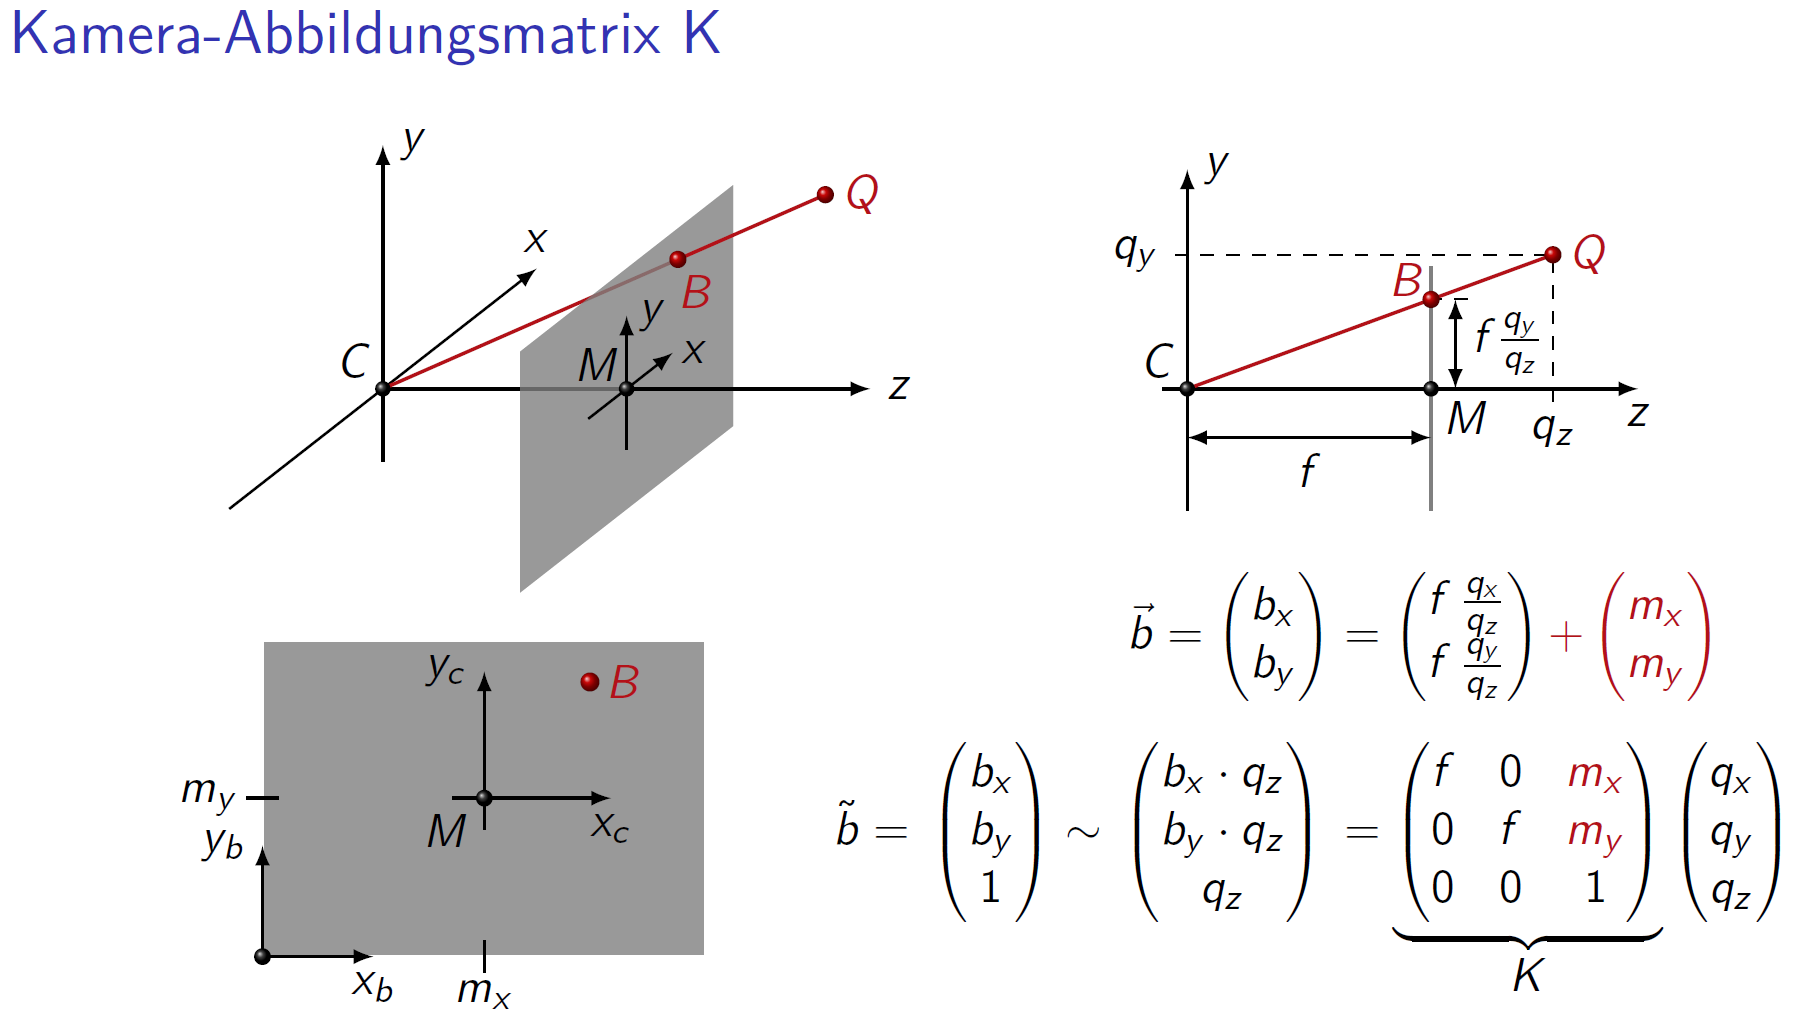
\includegraphics[width=0.9\linewidth]{Bilder/kamera1} \\
		 
		 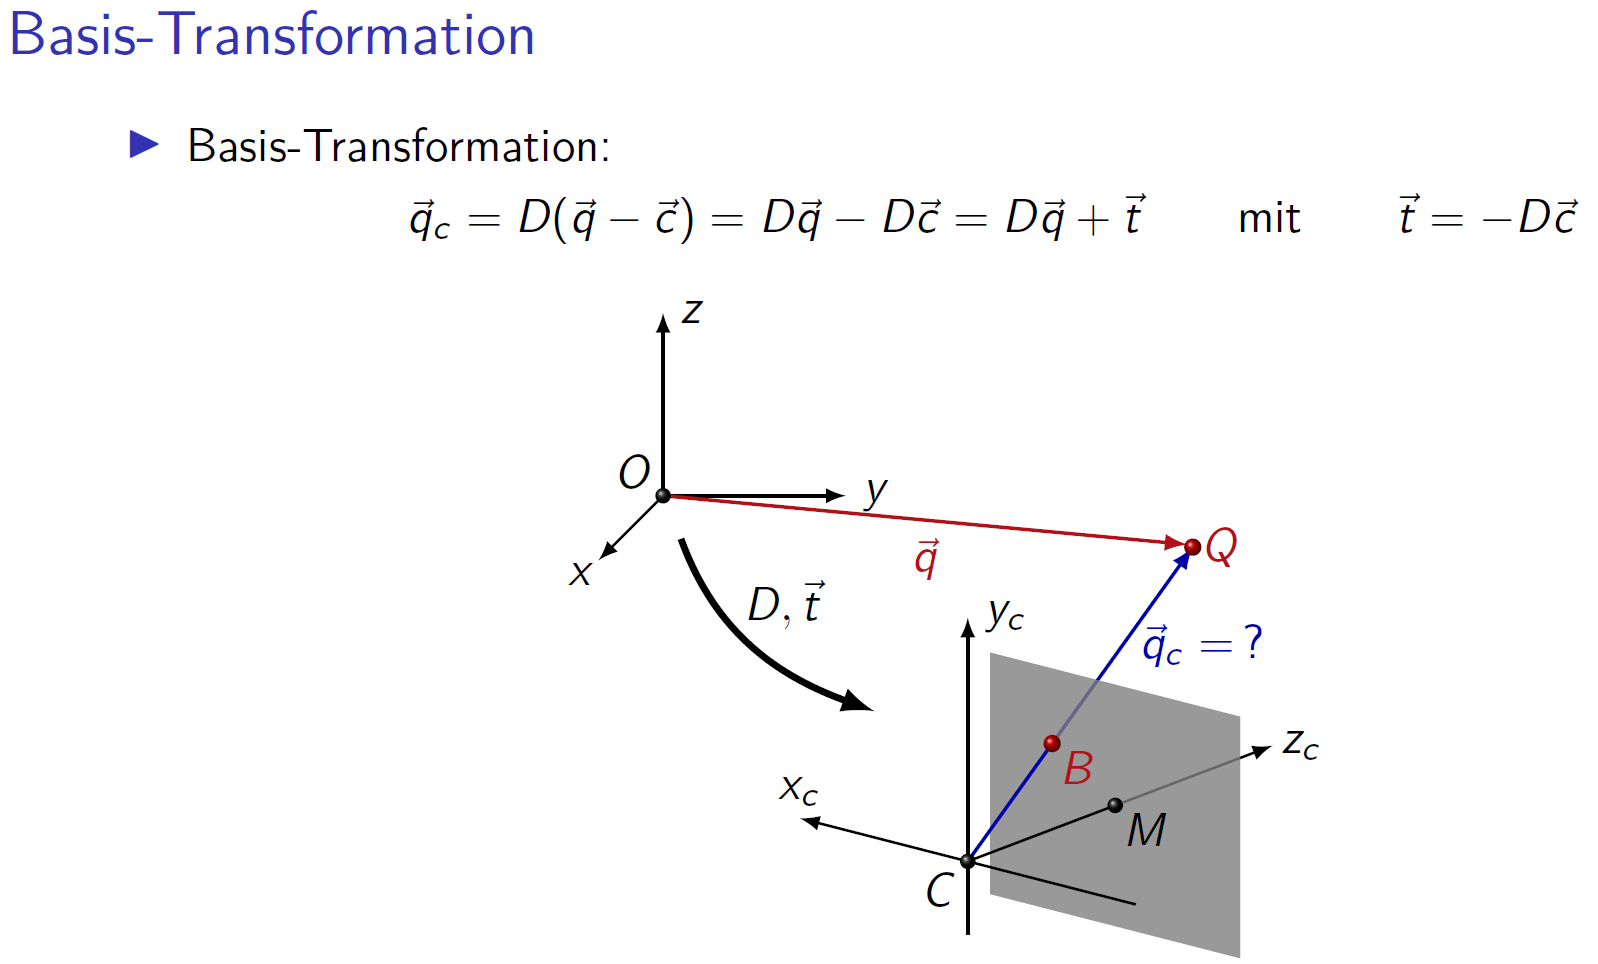
\includegraphics[width=0.9\linewidth]{Bilder/kamera2} \\
		 
		 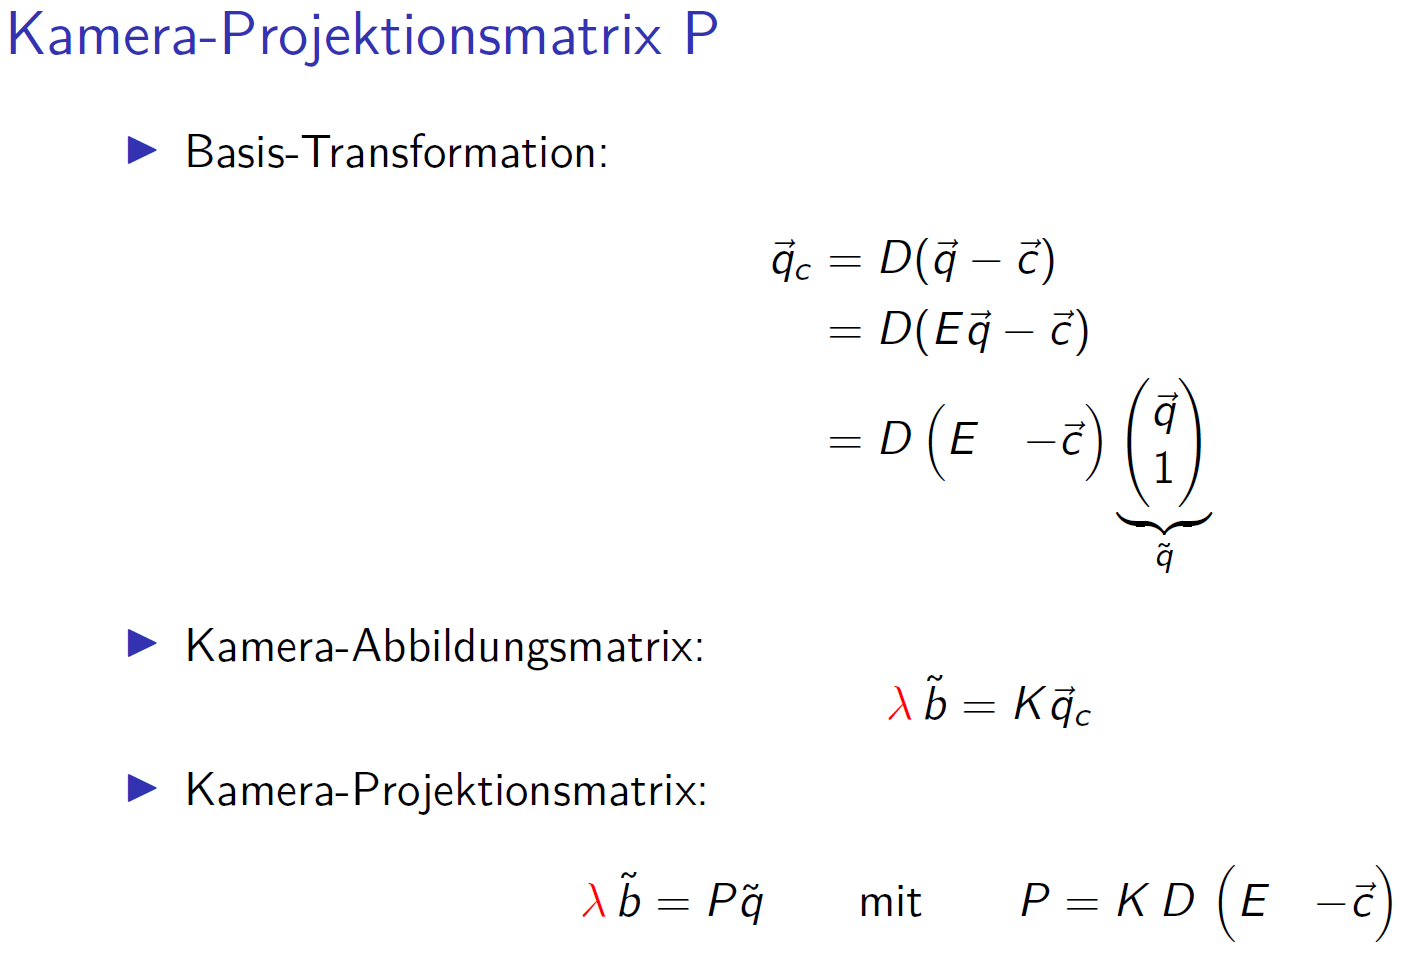
\includegraphics[width=0.9\linewidth]{Bilder/kamera3} \\
		 
		 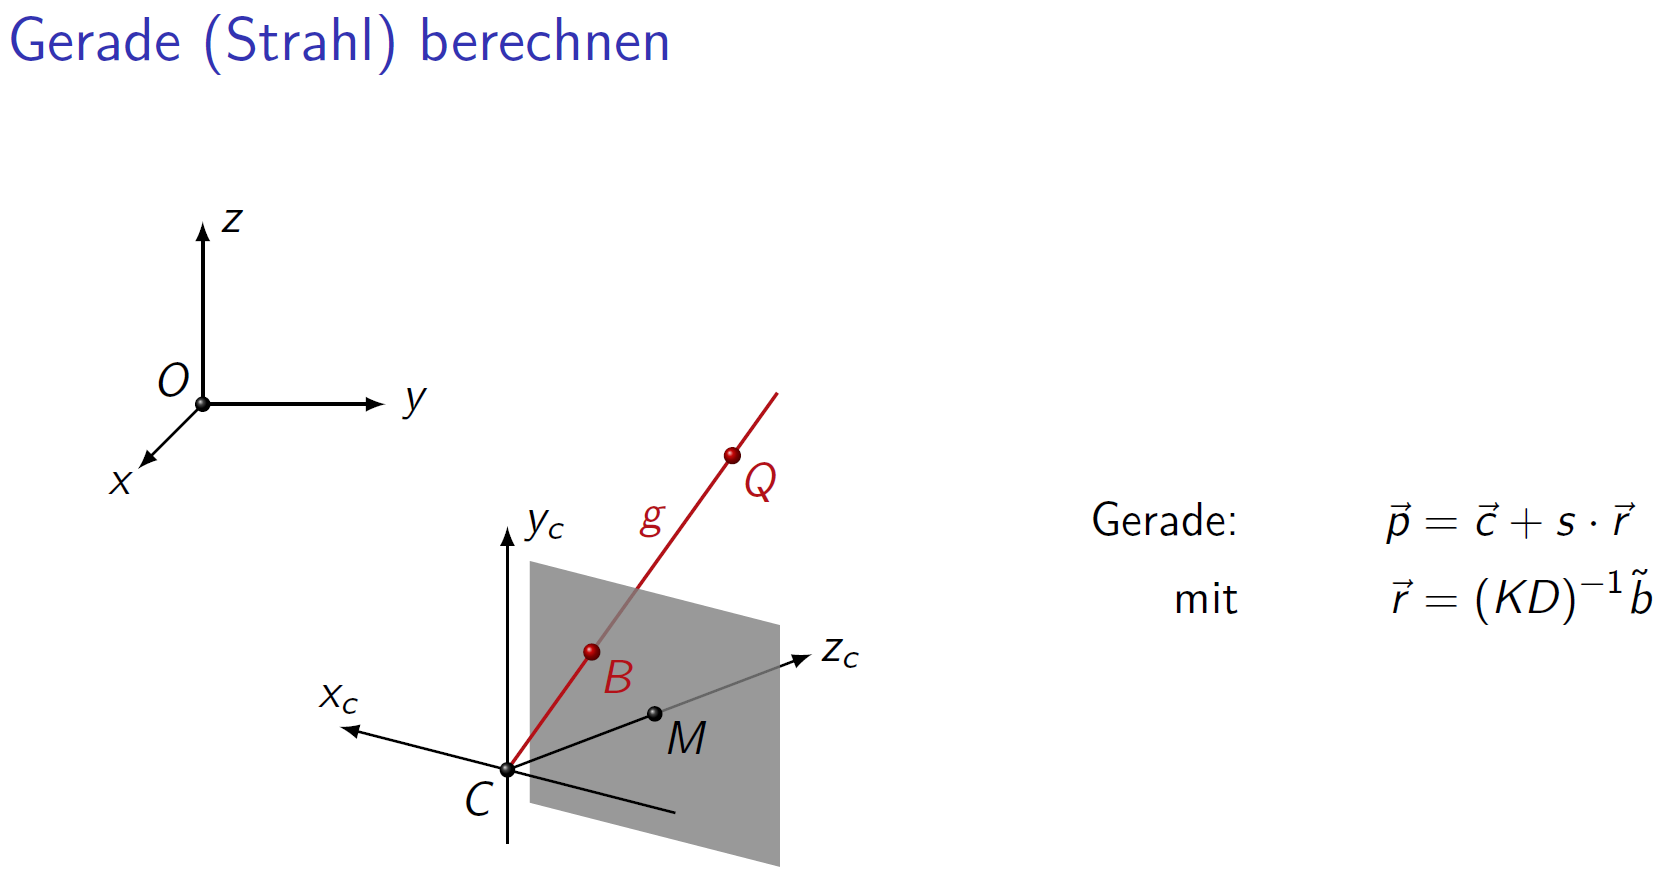
\includegraphics[width=0.9\linewidth]{Bilder/kamera4} 	 

	\subsection{Widerstandsnetzwerk}
		   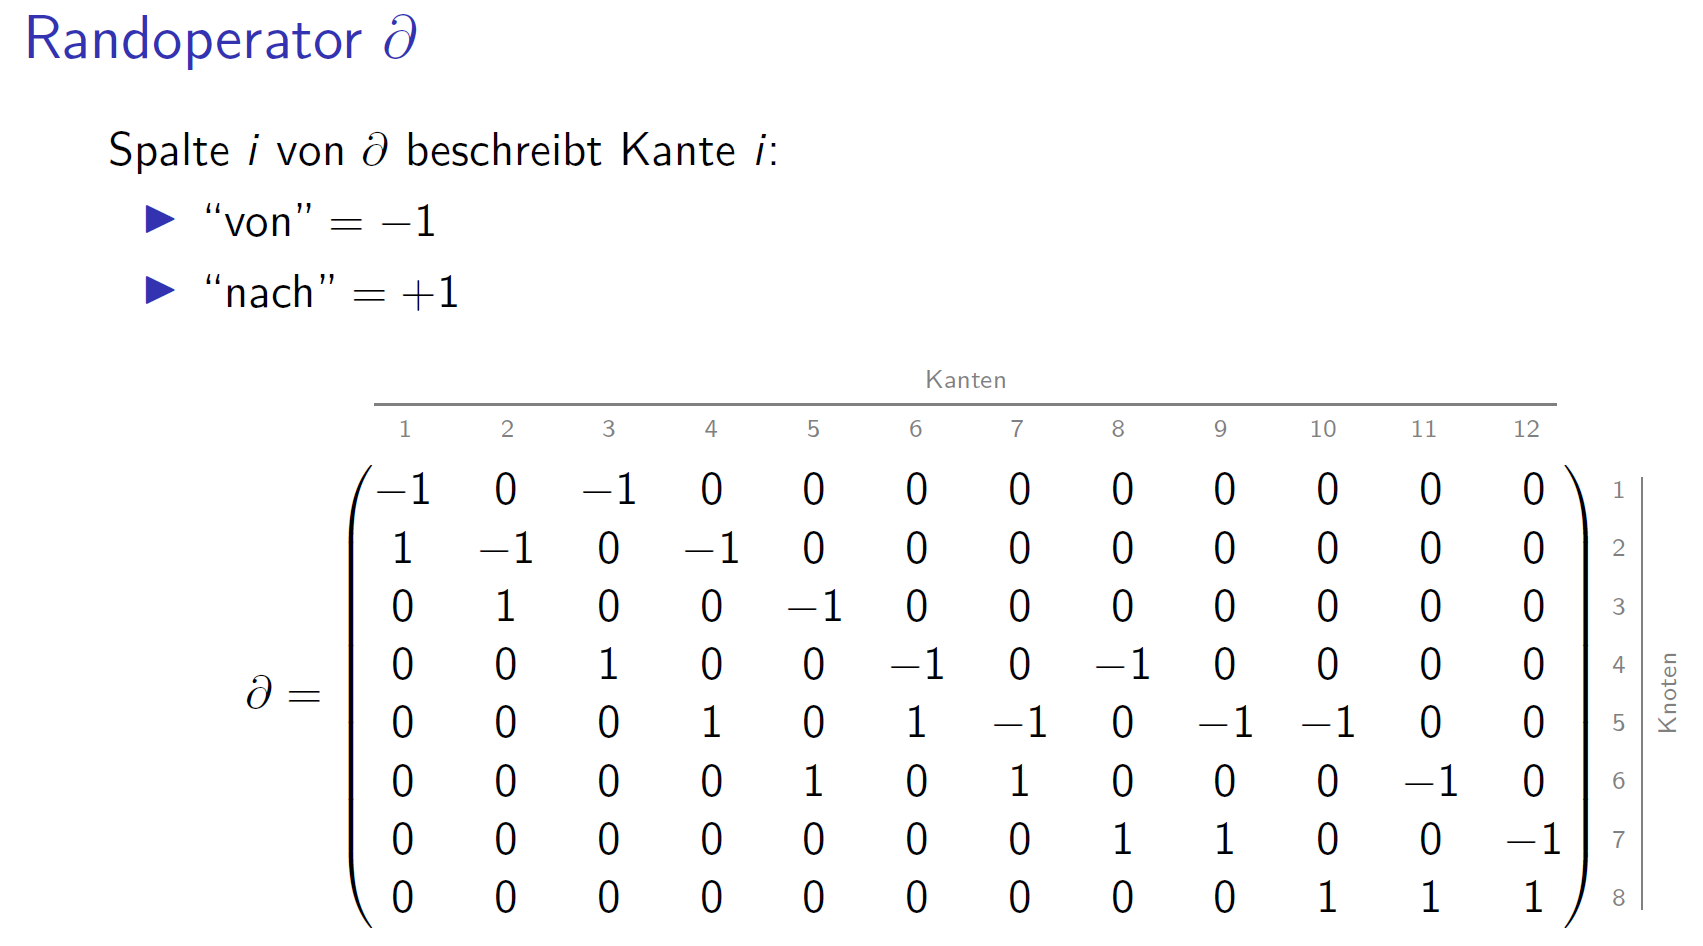
\includegraphics[width=0.8\linewidth]{Bilder/widerstand2} \\ 
		   
		   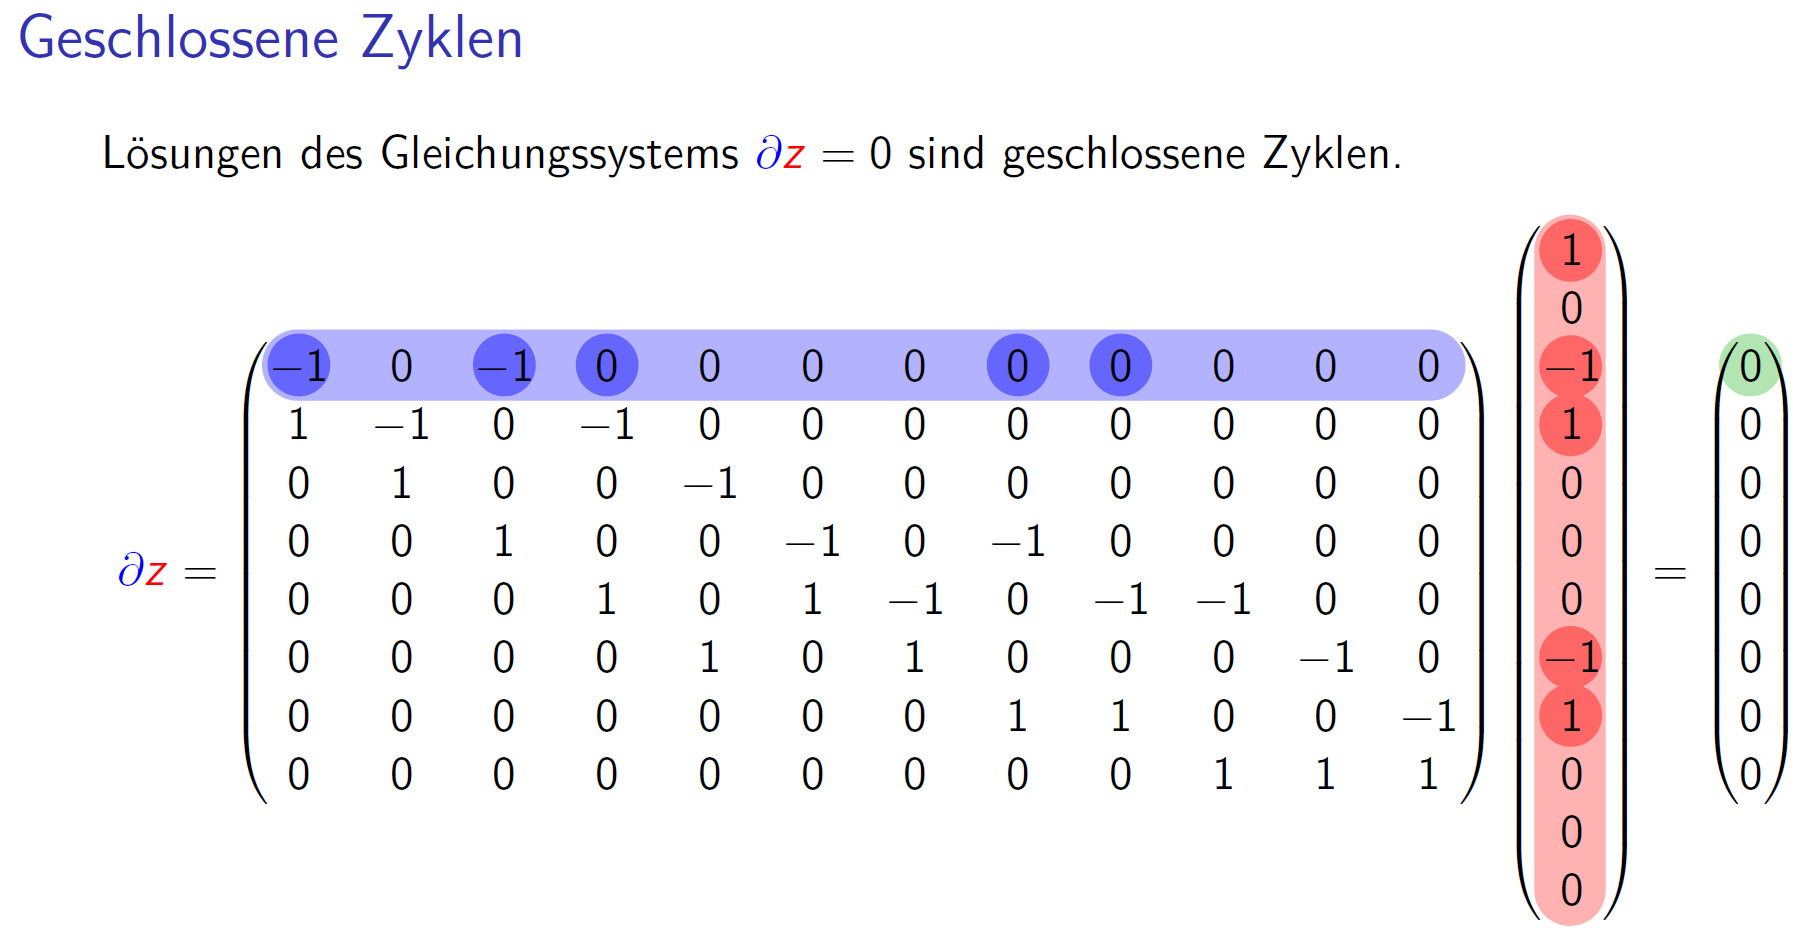
\includegraphics[width=0.8\linewidth]{Bilder/widerstand3} \\ 
		   Roter Vektor: gewählter Zyklus\\
		   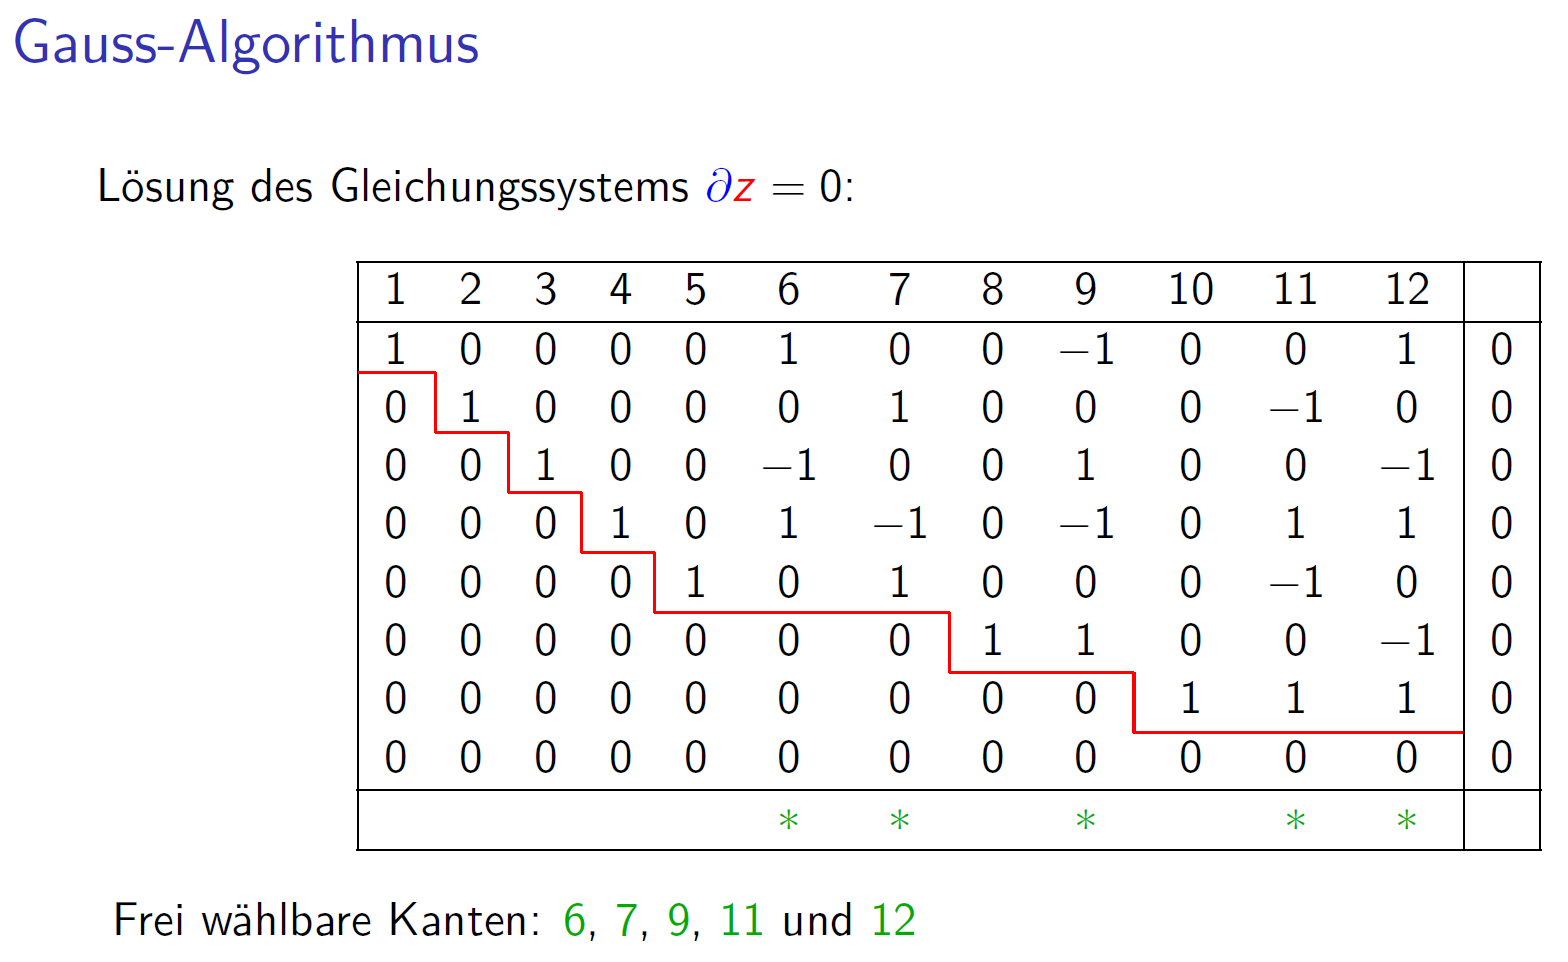
\includegraphics[width=0.8\linewidth]{Bilder/widerstand4} \\ 
		   
		   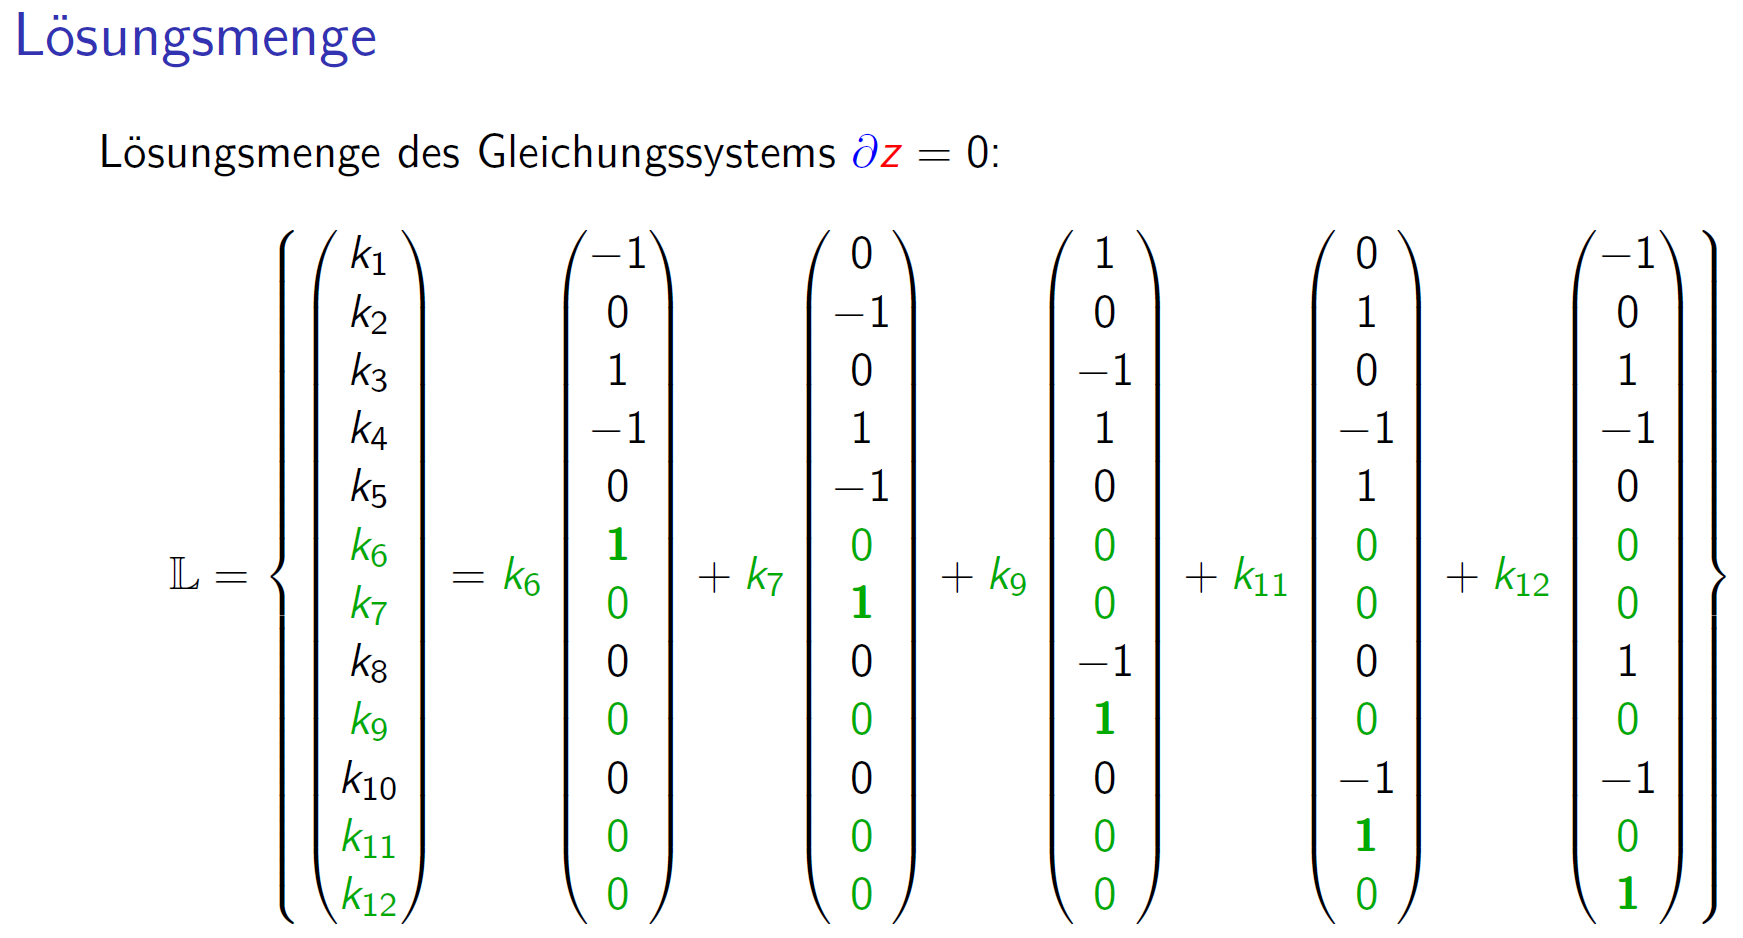
\includegraphics[width=0.8\linewidth]{Bilder/widerstand5} \\ 
	
	\subsection{Abbildungsmatrix}
		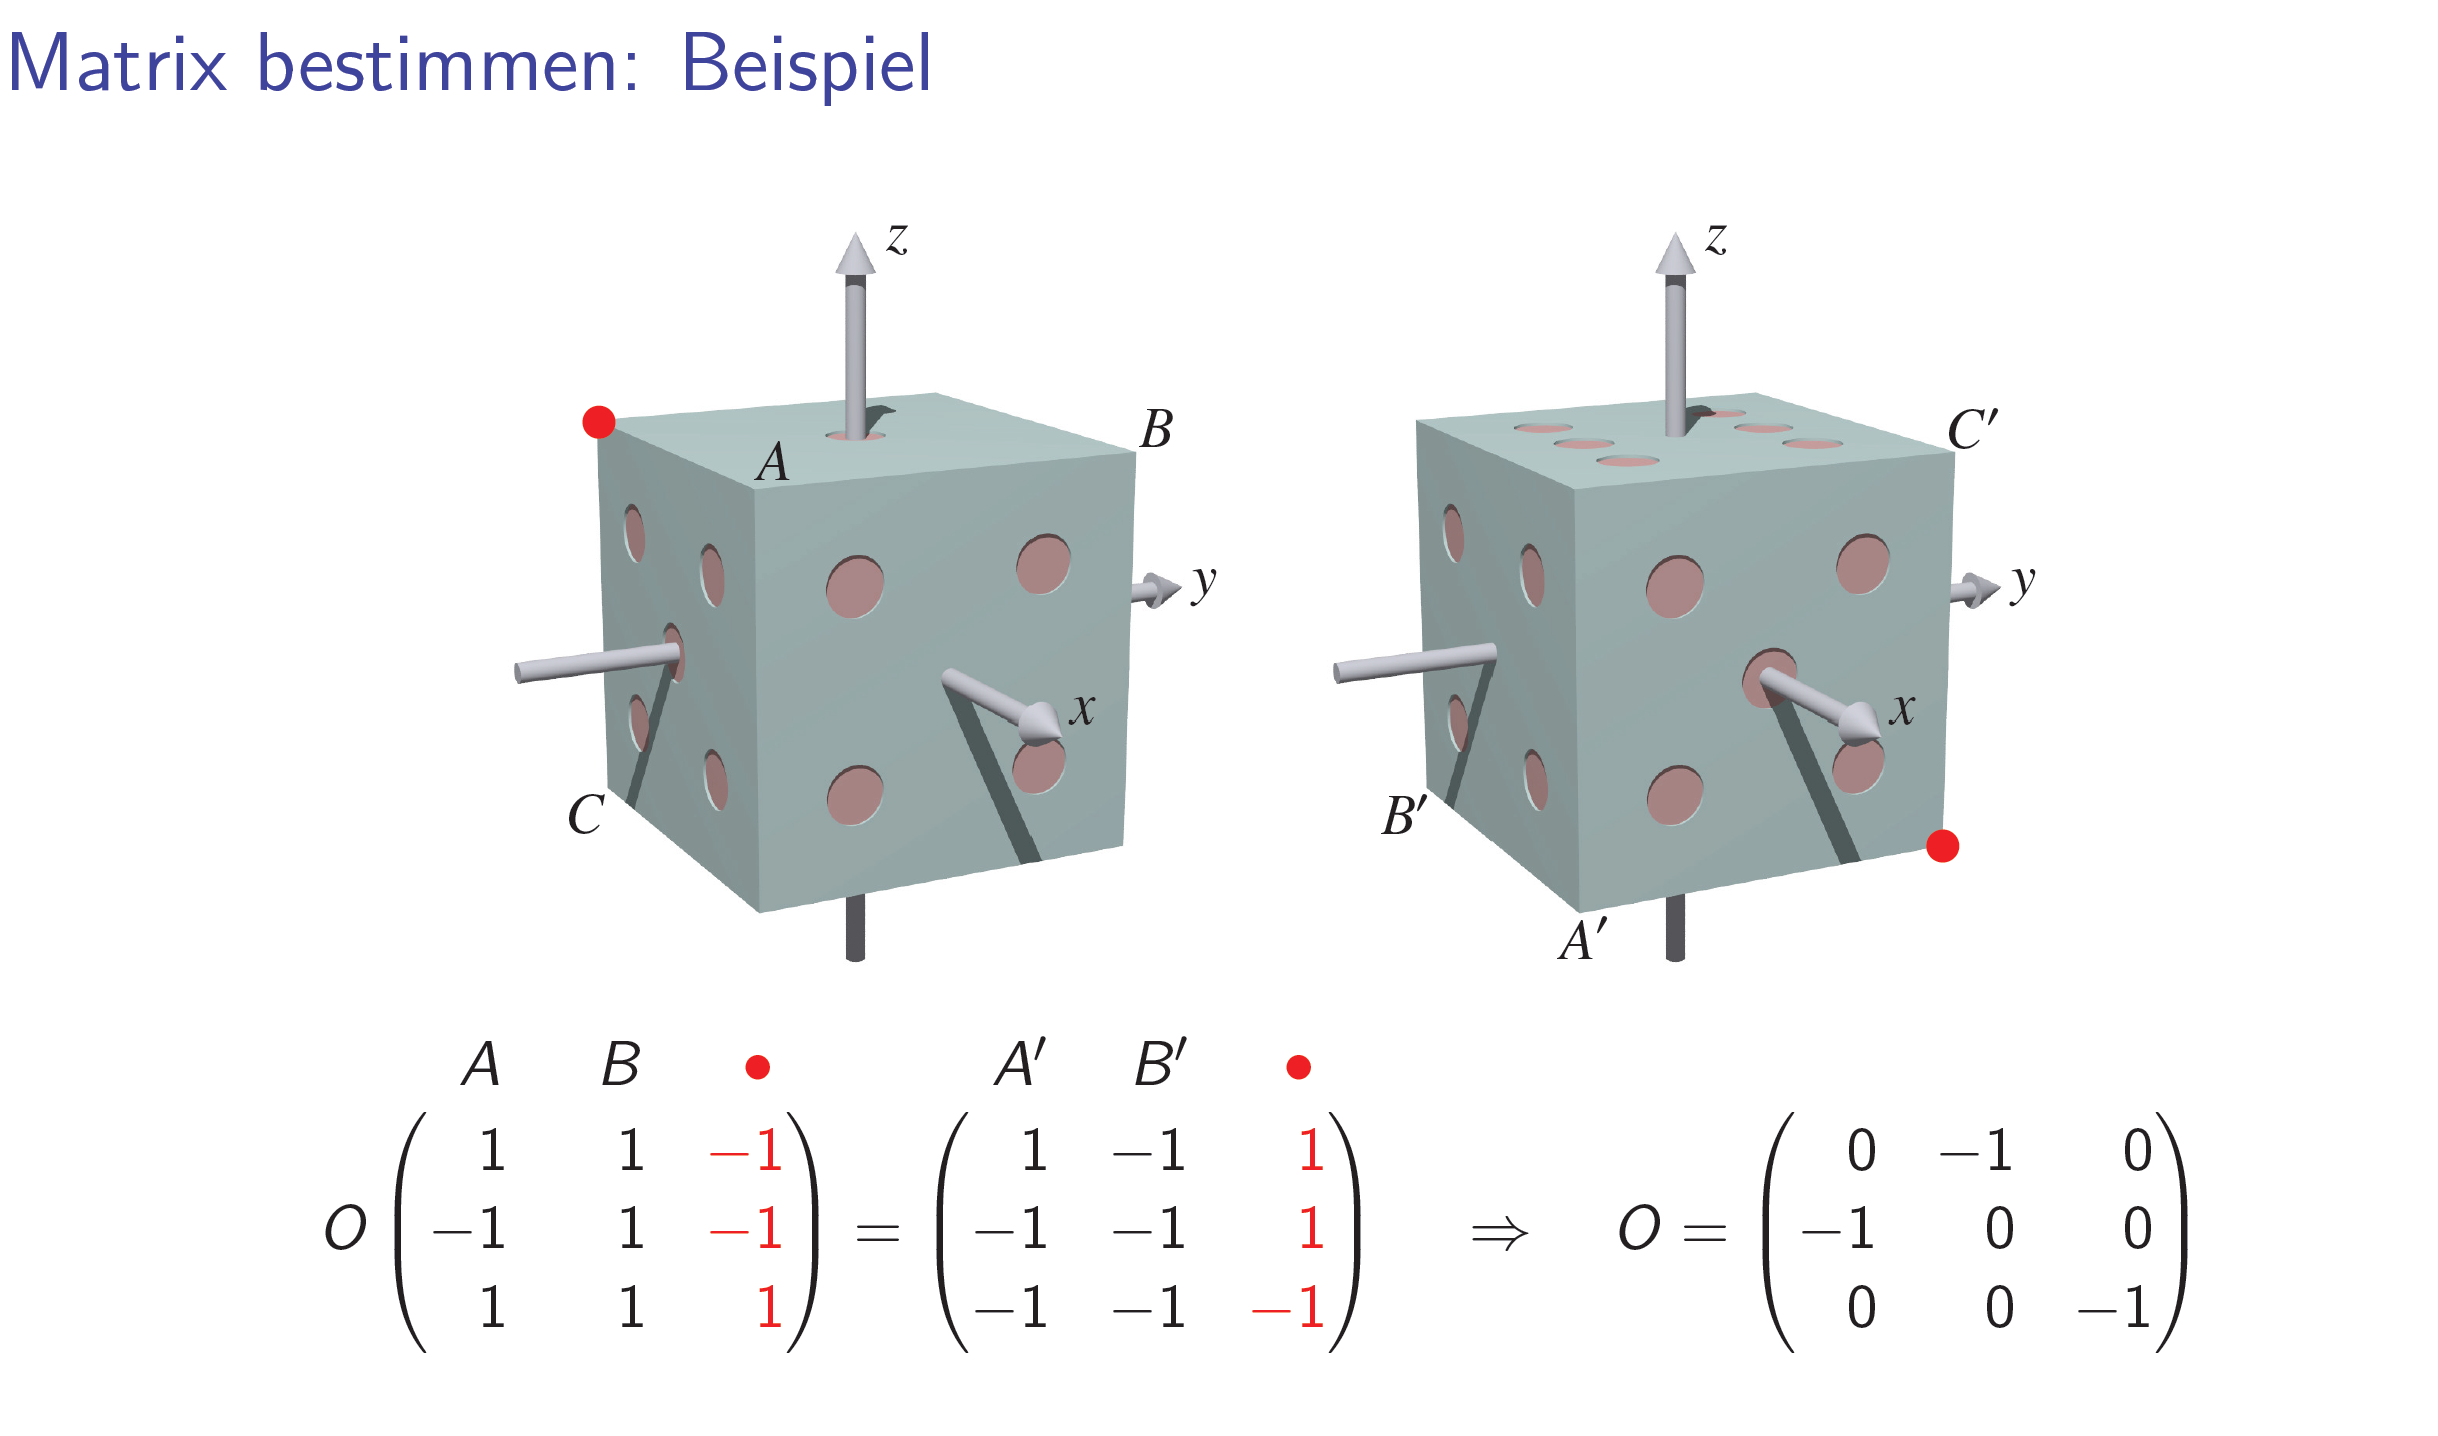
\includegraphics[width=0.8\linewidth]{Bilder/matrix-bestimmen_wuerfel-drehen.png} \\ 